%%%%%%%%%%%%%%%%%%%%%%%%%%%%%%%%%%%%%%%%%%%%%%%%%%%%%%%%%%%%%%%%%%%%%%%%%%%%%%%%
%% Plantilla de memoria en LaTeX para la ETSIT - Universidad Rey Juan Carlos
%%
%% Por Gregorio Robles <grex arroba gsyc.urjc.es>
%%     Grupo de Sistemas y Comunicaciones
%%     Escuela Técnica Superior de Ingenieros de Telecomunicación
%%     Universidad Rey Juan Carlos
%% (muchas ideas tomadas de Internet, colegas del GSyC, antiguos alumnos...
%%  etc. Muchas gracias a todos)
%%
%% La última versión de esta plantilla está siempre disponible en:
%%     https://github.com/gregoriorobles/plantilla-memoria
%%
%% Para obtener PDF, ejecuta en la shell:
%%   make
%% (las imágenes deben ir en PNG o JPG)

%%%%%%%%%%%%%%%%%%%%%%%%%%%%%%%%%%%%%%%%%%%%%%%%%%%%%%%%%%%%%%%%%%%%%%%%%%%%%%%%

\documentclass[a4paper, 12pt]{book}
%\usepackage[T1]{fontenc}

\usepackage{comment}
\usepackage{pdfpages}
\usepackage{subfig}
\usepackage{longtable}
\usepackage{multirow}
\usepackage{listings}
\usepackage{verbatimbox}
\usepackage[a4paper, left=2.5cm, right=2.5cm, top=3cm, bottom=3cm]{geometry}
\usepackage{times}
\usepackage[utf8]{inputenc}
\usepackage[spanish]{babel} % Comenta esta línea si tu memoria es en inglés
\usepackage{url}
%\usepackage[dvipdfm]{graphicx}
\usepackage{graphicx}
\usepackage{float}  %% H para posicionar figuras
\usepackage[nottoc, notlot, notlof, notindex]{tocbibind} %% Opciones de índice
\usepackage{latexsym}  %% Logo LaTeX

\title{Memoria ExChecker}
\author{Adrián Omar Riao Monsalve}

\renewcommand{\baselinestretch}{1.5}  %% Interlineado

\begin{document}

\renewcommand{\refname}{Bibliografía}  %% Renombrando
\renewcommand{\appendixname}{Apéndice}

%%%%%%%%%%%%%%%%%%%%%%%%%%%%%%%%%%%%%%%%%%%%%%%%%%%%%%%%%%%%%%%%%%%%%%%%%%%%%%%%
% PORTADA

\begin{titlepage}
\begin{center}

\includegraphics[scale=0.8]{img/URJ_logo_Color_POS.png}

\vspace{1.75cm}

\Large
GRADO EN INGENIERÍA EN TECNOLOGÍAS
DE LA TELECOMUNICACIÓN

\vspace{0.4cm}

\large
Curso Académico 2020/2021

\vspace{0.8cm}

Trabajo Fin de Grado

\vspace{2.5cm}

\LARGE
\textit{ExChecker}: Aplicación web para
corrección de exámenes tipo test con tecnología
OMR

\vspace{4cm}

\large
Autor : Adrián Omar Riao Monsalve\\
Tutor : Miguel Ángel Ortuño Pérez
\end{center}
\end{titlepage}

\newpage
\mbox{}
\thispagestyle{empty} % para que no se numere esta pagina


%%%%%%%%%%%%%%%%%%%%%%%%%%%%%%%%%%%%%%%%%%%%%%%%%%%%%%%%%%%%%%%%%%%%%%%%%%%%%%%%
%%%% Para firmar
\clearpage
\pagenumbering{gobble}
\chapter*{}

\vspace{-4cm}
\begin{center}
\LARGE
\textbf{Trabajo Fin de Grado}

\vspace{1cm}
\large
\textit{ExChecker}: Aplicación Web para
Corrección de Exámenes Tipo Test con Tecnología
OMR (Optical Mark Recognition)

\vspace{1cm}
\large
\textbf{Autor :} Adrián Omar Riao Monsalve \\
\textbf{Tutor :} Miguel Ángel Ortuño Pérez

\end{center}

\vspace{1cm}
La defensa del presente Proyecto Fin de Carrera se realizó el día \qquad$\;\,$ de \qquad\qquad\qquad\qquad \newline de 202X, siendo calificada por el siguiente tribunal:


\vspace{0.5cm}
\textbf{Presidente:}

\vspace{1.2cm}
\textbf{Secretario:}

\vspace{1.2cm}
\textbf{Vocal:}


\vspace{1.2cm}
y habiendo obtenido la siguiente calificación:

\vspace{1cm}
\textbf{Calificación:}


\vspace{1cm}
\begin{flushright}
Fuenlabrada, a \qquad$\;\,$ de \qquad\qquad\qquad\qquad de 202X
\end{flushright}

%%%%%%%%%%%%%%%%%%%%%%%%%%%%%%%%%%%%%%%%%%%%%%%%%%%%%%%%%%%%%%%%%%%%%%%%%%%%%%%%
%%%% Dedicatoria

\chapter*{}
\pagenumbering{Roman} % para comenzar la numeracion de paginas en numeros romanos
\begin{flushright}
\textit{Dedicado a \\
Santiago, por ser el primero en
enseñarme que el conocimiento es poder}
\end{flushright}

%%%%%%%%%%%%%%%%%%%%%%%%%%%%%%%%%%%%%%%%%%%%%%%%%%%%%%%%%%%%%%%%%%%%%%%%%%%%%%%%
%%%% Agradecimientos

\chapter*{Agradecimientos}
%\addcontentsline{toc}{chapter}{Agradecimientos} % si queremos que aparezca en el índice
\markboth{AGRADECIMIENTOS}{AGRADECIMIENTOS} % encabezado 

Todo esfuerzo tiene su recompensa. Estas palabras han formado parte de
mi bagaje todos estos años, y hoy más que nunca, es cuando más sentido
les doy.

Me gustaría aprovechar estas breves líneas para agradecer a aquellos que
me han transmitido su conocimiento. Personas que, apasionados por su
trabajo, brindan tiempo, dedicación y esfuerzo a aquellos que lo necesitan.
Gracias a ellos hoy soy uno más.

En segundo lugar, agradecer a mis amigos, compañeros de vida, 
y a mi pareja por la honestidad,
el respeto, y sobre todo el positivismo adoptado ante situaciones adversas.
Sin su apoyo ahora mismo no estaría escribiendo estas palabras.

Me gustaría dar las gracias a la Universidad Rey Juan Carlos por brindarme
tal oportunidad de formación, así como a mi tutor de proyecto Miguel
Ángel Ortuño Pérez por los recursos
ofrecidos y su ayuda inmediata en cuanto la he necesitado. He sido muy
afortunado al poder formarme en una institución altamente cualificada para
el desarrollo de actividades en su campo, y que cuenta con un gran número
de profesionales a los que, con indiscutible orgullo, he tenido el placer
de conocer.

Por último, me gustaría agradecer a mis padres la confianza que siempre
han depositado en mí. Gracias a su apoyo, compromiso y paciencia hoy puedo
decir que estoy orgulloso de la persona en la que me he convertido.

%%%%%%%%%%%%%%%%%%%%%%%%%%%%%%%%%%%%%%%%%%%%%%%%%%%%%%%%%%%%%%%%%%%%%%%%%%%%%%%%
%%%% Resumen

\chapter*{Resumen}
%\addcontentsline{toc}{chapter}{Resumen} % si queremos que aparezca en el índice
\markboth{RESUMEN}{RESUMEN} % encabezado

\begin{comment}
Los exámenes tipo test como método de evaluación de conocimientos en
alumnos son muy utilizados actualmente. Esto es así debido a que son
fáciles de elaborar y de corregir. Aún así, se puede utilizar un
proceso de automatización en esta corrección, de forma que a los
evaluadores le resulte más fácil y sencillo este proceso de corrección.

En la actualidad existen técnicas que automatizan estos procesos, como
máquinas físicas que detectan marcas en los documentos o aplicaciones
que utilizan tecnología OMR (Optical Mark Recognition). En este último
caso las aplicaciones que encontramos son muy pocas, y su funcionamiento
no está lo suficientemente pulido. Por estas razones, el objetivo de
este proyecto es desarrollar una aplicación web que, utilizando la
tecnología OMR, sea capaz de corregir exámenes tipo test de forma
automática.
\end{comment}

Los exámenes tipo test como método de evaluación de conocimientos en
alumnos son muy utilizados actualmente. Esto es así debido a que son
fáciles de elaborar y de corregir. Aún así, se puede utilizar un
proceso de automatización en esta corrección, de forma que a los
evaluadores le resulte más fácil y sencillo este proceso de corrección.
En la actualidad existen técnicas que automatizan estos procesos, como
la tecnología OMR (Optical Mark Recognition).

El objetivo de este proyecto es desarrollar una aplicación
web que, utilizando la tecnología OMR ya existente,
sea capaz de corregir exámenes tipo
test de forma automática. En otras palabras, desarrollaremos un \textit{frontend}
para un sistema OMR proporcionado por el usuario \textit{Udayraj123} en
\textit{Github}\footnote{https://github.com/Udayraj123/OMRChecker}.
La aplicación web estará orientada a educación secundaria y
dará la posibilidad de
introducir en el sistema los exámenes a corregir escaneados o
fotografiados. Estos exámenes serán realizados en papel, ya que hay muchos
entornos donde no hay ordenadores para
todos los alumnos todo el tiempo. De esta manera, aunque el profesor
no disponga de un escáner, será capaz de corregir los exámenes utilizando
su dispositivo móvil.

Para llevar a cabo este desarrollo se ha utilizado el lenguaje \textit{Python}
y un \textit{framework} web disponible en este lenguaje llamado \textit{Django}. 
Gracias
a esto hemos desarrollado una aplicación web totalmente responsiva que
permite a sus usuarios la generación de plantillas de exámenes tipo
test y su posterior corrección subiendo los documentos a la plataforma.
Además se han utilizado tecnologías de subida de documentos en web,
como la librería \textit{Filepond}, y distintas herramientas para 
la generación de plantillas, como \textit{Wkhtmltopdf}, \textit{Pdfkit} o \textit{Jinja2}.

Este proyecto ha sido desarrollado con el objetivo de realizar
un despliegue con la herramienta
\textit{Docker}, de forma que los usuarios pueden instalar la aplicación
en su equipo local para así ejecutarla y acceder a ella. Es importante destacar
que al presentarse la aplicación en un contenedor de \textit{Docker} ésta puede
ser ejecutada desde Windows, Linux o Mac.

%%%%%%%%%%%%%%%%%%%%%%%%%%%%%%%%%%%%%%%%%%%%%%%%%%%%%%%%%%%%%%%%%%%%%%%%%%%%%%%%
%%%% Resumen en inglés

\chapter*{Summary}
%\addcontentsline{toc}{chapter}{Summary} % si queremos que aparezca en el índice
\markboth{SUMMARY}{SUMMARY} % encabezado

Multiple choice exams as a method of evaluating knowledge in
students are widely used today. This is so because they are easy
to make and correct. Still, an automation process can be used in
this correction, making this correction process easier and easier
for evaluators. Currently there are techniques that automate these
processes, such as OMR (Optical Mark Recognition) technology.

The objective of this project is to develop a web application that,
using OMR technology, is capable of correcting multiple choice
exams automatically. In other words, we will develop a frontend
for an OMR system provided by \textit{Udayraj123} on
\textit{Github}\footnote{https://github.com/Udayraj123/OMRChecker}.
The web application will be oriented to secondary education and
It will give the possibility of
entering the scanned exams or photographed exams into the
system to be corrected. These exams will be done on paper, as
there are many environments where there are not computers
for all students all the time. In this way, even if the teacher does
not have a scanner, he will be able to correct the exams using his
mobile device.

To carry out this development, the \textit{Python} language has been used
and a web \textit{framework} available in this language called \textit{Django}.
Thanks to this we have developed a fully responsive web application
that allows its users to generate multiple choice exam templates
and their subsequent correction by uploading the documents to
the platform. In addition, there are many technologies that have been used for
uploading documents on the web, such as the \textit{Filepond} library,
and different tools for generating templates, such as \textit{Wkhtmltopdf},
\textit{Pdfkit} or \textit{Jinja2}.

This project has been developed with the aim of carrying out
a deployment with the \textit{Docker} tool, so that users can install
the application on their local machine in order to run and
access it. The web application is
presented in a \textit{Docker} container, so it can be run from Windows, Linux or Mac.


%%%%%%%%%%%%%%%%%%%%%%%%%%%%%%%%%%%%%%%%%%%%%%%%%%%%%%%%%%%%%%%%%%%%%%%%%%%%%%%%
%%%%%%%%%%%%%%%%%%%%%%%%%%%%%%%%%%%%%%%%%%%%%%%%%%%%%%%%%%%%%%%%%%%%%%%%%%%%%%%%
% ÍNDICES %
%%%%%%%%%%%%%%%%%%%%%%%%%%%%%%%%%%%%%%%%%%%%%%%%%%%%%%%%%%%%%%%%%%%%%%%%%%%%%%%%

% Las buenas noticias es que los índices se generan automáticamente.
% Lo único que tienes que hacer es elegir cuáles quieren que se generen,
% y comentar/descomentar esa instrucción de LaTeX.

%%%% Índice de contenidos
\tableofcontents 
%%%% Índice de figuras
\cleardoublepage
%\addcontentsline{toc}{chapter}{Lista de figuras} % para que aparezca en el indice de contenidos
\listoffigures % indice de figuras
%%%% Índice de tablas
\cleardoublepage
%\addcontentsline{toc}{chapter}{Lista de tablas} % para que aparezca en el indice de contenidos
\listoftables % indice de tablas


%%%%%%%%%%%%%%%%%%%%%%%%%%%%%%%%%%%%%%%%%%%%%%%%%%%%%%%%%%%%%%%%%%%%%%%%%%%%%%%%
%%%%%%%%%%%%%%%%%%%%%%%%%%%%%%%%%%%%%%%%%%%%%%%%%%%%%%%%%%%%%%%%%%%%%%%%%%%%%%%%
% INTRODUCCIÓN %
%%%%%%%%%%%%%%%%%%%%%%%%%%%%%%%%%%%%%%%%%%%%%%%%%%%%%%%%%%%%%%%%%%%%%%%%%%%%%%%%

\cleardoublepage
\chapter{Introducción}
\label{sec:intro} % etiqueta para poder referenciar luego en el texto con ~\ref{sec:intro}
\pagenumbering{arabic} % para empezar la numeración de página con números

En este capítulo introduciremos información general relativa al proyecto
que sirva de introducción al lector. De esta manera nos aproximaremos a los
objetivos, requisitos y tecnologías que se referencian en esta memoria.

\section{Contexto}
\label{sec:Contexto}

Estos últimos años hemos vivido una transformación digital
importante. En cuestión de décadas, el ámbito de la informática, las
telecomunicaciones, y la ciencia han experimentado un crecimiento
de desarrollo prácticamente exponencial. Gracias a esto, podemos disfrutar
de un ecosistema tecnológico bastante amplio, teniendo la oportunidad como
usuarios de ser partícipes en esta evolución y utilizar un sinfín de
tecnologías propuestas con el objetivo de beneficiar la vida de las personas.
En este sentido, los requisitos de los usuarios cada vez son más exigentes,
y allá donde exista un problema a nivel global las tecnologías deben proponer
soluciones para intentar erradicarlo.

Aún siendo esta la intención, existen algunos ámbitos sociales en los que la
tecnología no ha arraigado de una manera tan profunda. Observamos que aún queda
mucho trabajo de realización, desarrollo y concienciación.

El ámbito de la enseñanza es un claro ejemplo en el que siguen existiendo
mecanismos y políticas bastante ligadas a épocas anteriores. Esto es un
problema a día de hoy, ya que como hemos comentado, nuevas tecnologías se
van implantando y cogen el relevo de las anteriores. De esta manera, cuestiones
como la enseñanza online, planificación temporal y/o corrección de exámenes
son prácticamente ejecutables en un menor tiempo y esfuerzo, evaluando las
mismas capacidades y cualidades del alumnado.


\section{Motivación}
\label{sec:Motivación}

En la actualidad existen muchas maneras de evaluar distintos conocimientos,
capacidades y cualidades del alumnado. Desde participación en clase hasta
pruebas teórico/prácticas. Todas ellas son perfectamente aceptables, aunque
existe desde hace unos años un debate abierto de cómo mejorar estas técnicas
de enseñanza y evaluación. Estas son algunas preguntas que se manifiestan
en este tipo de debates:

\begin{itemize}
  \item ¿Qué contenidos deberían llevar las pruebas teóricas?
  
  \item ¿Cómo administrar información al alumno de una forma eficiente?
  
  \item ¿Cuál debería ser la planificación temporal adecuada?
\end{itemize}

\subsection{Exámenes tipo test}
\label{subsec:examenes_tipo_test}

Los exámenes tipo test en el ámbito educativo han sido una técnica bastante
utilizada por los profesores debido a varias razones.

\begin{itemize}
  \item Son fáciles de realizar y de corregir.

  \item Ahorran mucho tiempo al profesor en la realización y corrección.
  
  \item Se puede cubrir muchas áreas de contenido en un único examen
  y aún así ser respondido en un corto período de tiempo.
\end{itemize}

Una característica básica de este tipo de exámenes es que la corrección
es totalmente objetiva, es decir, un examen tipo test que conste de cuatro respuestas
por pregunta únicamente tendrá una respuesta correcta en esas cuatro opciones 
(suponiendo, claro está, que el examen no permite la respuesta múltiple).
De esta manera, si el examen es corregido por dos profesores cualesquiera la
calificación final debe ser igual.
Para cumplir esta propiedad es necesario que el examen tipo test se haya
confeccionado especialmente para que sea lo más objetivo posible.

Gracias a esta propiedad de los exámenes tipo test nos damos cuenta de una
particularidad. ¡Un ordenador también podría corregir un examen tipo test!
Y sería bastante sencillo, únicamente tendríamos que aportarle información
de qué respuestas son válidas y cuáles no. El ordenador estaría capacitado
para realizar este cálculo, y en el caso de aportarle información adicional
como la nota máxima del examen, penalización por respuesta fallida,
opción de respuesta múltiple... sería lo suficientemente autónomo como para
devolvernos los resultados deseados.

Actualmente existen programas informáticos que realizan estas correcciones
de exámenes tipo test. Los profesores generalmente obtienen una plantilla
que reconoce el propio sistema y los exámenes son corregidos automáticamente.
De esta forma, un profesor únicamente se debe de preocupar de redactar el
examen.

Existen soluciones comerciales completas, con hardware dedicado que
se ocupan de estas correcciones, pero su precio
suele ser bastante elevado y sobre todo están ligadas a un lugar específico.
Esto quiere decir que si un profesor desea corregir sus exámenes desde su
domicilio no podría hacerlo. También existen aplicaciones online que
utilizan este sistema para la corrección de exámenes. Aún así, estas
herramientas no están lo suficientemente pulidas y son muy básicas. 

\subsection{Tecnología OMR (Optical Mark Recognition)}
\label{subsec:tecnologia_omr}

La tecnología OMR (Optical Mark Recognition) es la tecnología que se encarga
del proceso de captura de datos de marcas desde documentos en papel. 
Esta tecnología se desarrolla mediante programas informáticos, 
sin embargo, en un inicio,
únicamente estaba implementada en dispositivos físicos que tenían que ser
adquiridos por los usuarios.
Debido al alto coste económico de estos equipos se hizo evidente la
necesidad de búsqueda de otras implementaciones.

Un precursor del OMR fueron las tarjetas perforadas, que se utilizaban como
dispositivos de entrada para las computadoras. En este caso se utilizaba
el uso de agujeros en vez de marcas de tinta en la superficie.
Este uso decayó rápidamente con la introducción de los ordenadores
personales.

En los sistemas OMR modernos, las presencias de pequeñas marcas de tinta son
reconocidas, y este reconocimiento se hace mediante un escáner óptico.
El código de barras o los códigos QR son tecnologías muy similares a esta.

\begin{comment}
\subsection{Estilo}
\label{subsec:estilo}

Recomiendo leer los consejos prácticos sobre escribir documentos científicos en \LaTeX \ de Diomidis Spinellis\footnote{\url{https://github.com/dspinellis/latex-advice}}.

Lee sobre el uso de las comas\footnote{\url{http://narrativabreve.com/2015/02/opiniones-de-un-corrector-de-estilo-11-recetas-para-escribir-correctamente-la-coma.html}}. 
Las comas en español no se ponen al tuntún.
Y nunca, nunca entre el sujeto y el predicado (p.ej. en ``Yo, hago el TFG'' sobre la coma).
La coma no debe separar el sujeto del predicado en una oración, pues se cortaría la secuencia natural del discurso.
No se considera apropiado el uso de la llamada coma respiratoria o \emph{coma criminal}.
Solamente se suele escribir una coma para marcar el lugar que queda cuando omitimos el verbo de una oración, pero es un caso que se da de manera muy infrecuente al escribir un texto científico (p.ej. ``El Real Madrid, campeón de Europa'').

A continuación, viene una figura, la Figura~\ref{figura:foro_hilos}. 
Observarás que el texto dentro de la referencia es el identificador de la figura (que se corresponden con el ``label'' dentro de la misma). 
También habrás tomado nota de cómo se ponen las ``comillas dobles'' para que se muestren correctamente. 
Nota que hay unas comillas de inicio (``) y otras de cierre (''), y que son diferentes.
Volviendo a las referencias, nota que al compilar, la primera vez se crea un diccionario con las referencias, y en la segunda compilación se ``rellenan'' estas referencias. 
Por eso hay que compilar dos veces tu memoria.
Si no, no se crearán las referencias.

 \begin{figure}
    \centering
    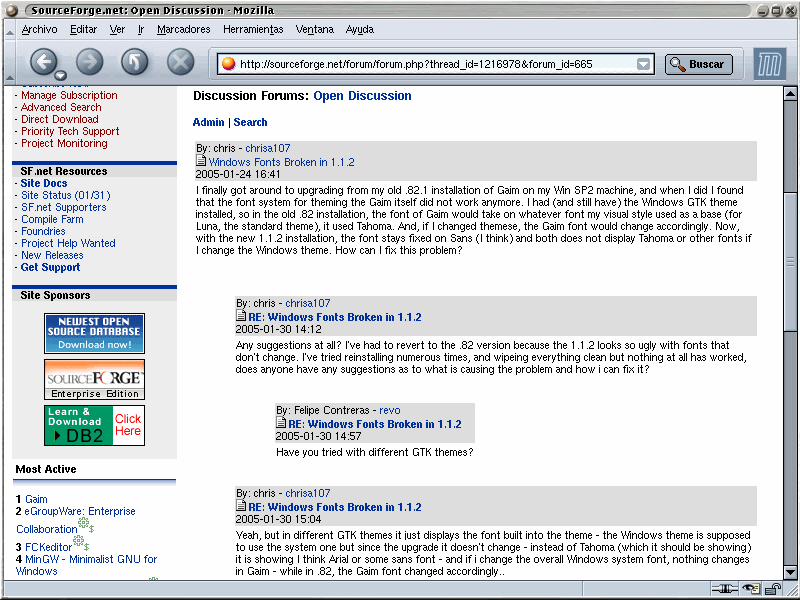
\includegraphics[bb=0 0 800 600, width=12cm, keepaspectratio]{img/foro1}
    \caption{Página con enlaces a hilos}
    \label{figura:foro_hilos}
 \end{figure}

A continuación un bloque ``verbatim'', que se utiliza para mostrar texto tal cual.
Se puede utilizar para ofrecer el contenido de correos electrónicos, código, entre otras cosas.

{\footnotesize
\begin{verbatim}
    From gaurav at gold-solutions.co.uk  Fri Jan 14 14:51:11 2005
    From: gaurav at gold-solutions.co.uk (gaurav_gold)
    Date: Fri Jan 14 19:25:51 2005
    Subject: [Mailman-Users] mailman issues
    Message-ID: <003c01c4fa40$1d99b4c0$94592252@gaurav7klgnyif>

    Dear Sir/Madam,
    How can people reply to the mailing list?  How do i turn off
    this feature? How can i also enable a feature where if someone
    replies the newsletter the email gets deleted?
    Thanks

    From msapiro at value.net  Fri Jan 14 19:48:51 2005
    From: msapiro at value.net (Mark Sapiro)
    Date: Fri Jan 14 19:49:04 2005
    Subject: [Mailman-Users] mailman issues
    In-Reply-To: <003c01c4fa40$1d99b4c0$94592252@gaurav7klgnyif>
    Message-ID: <PC173020050114104851057801b04d55@msapiro>

    gaurav_gold wrote:
    >How can people reply to the mailing list?  How do i turn off
    this feature? How can i also enable a feature where if someone
    replies the newsletter the email gets deleted?

    See the FAQ
    >Mailman FAQ: http://www.python.org/cgi-bin/faqw-mm.py
    article 3.11
\end{verbatim}
}
\end{comment}

\section{Estructura de la memoria}
\label{sec:estructura}

La memoria de este proyecto ha sido dividida en 6 capítulos. Procedemos
a explicar qué contenido del proyecto aborda cada capítulo.

En este primer capítulo nos centramos en explicar la motivación que nos
ha llevado a realizar este proyecto, partiendo del contexto en el que
nos encontramos y, de esta manera, situando el proyecto en una dimensión
espacial y temporal. Por consiguiente, se pretende dar una introducción al
lector para que se familiarice con el proyecto.

El segundo capítulo describirá los objetivos fundamentales de este proyecto.
Además, se presentará una planificación temporal del proyecto en sí.

En tercer lugar, el tercer capítulo comprende las tecnologías utilizadas en
el proyecto, indicando la razón de haber sido escogidas. A su vez, se
manifestará el peso que cada una de ellas posee en el proyecto, puntualizando
las características individuales de cada una.

En el cuarto capítulo es donde se explicará, de una manera más detallada,
el diseño y la implementación del proyecto. Se mostrará la arquitectura
propuesta y, sobre todo, se discutirán las razones de elección de diseño.
Adicionalmente, haremos referencia a un punto bastante importante del
proyecto: el despliegue de nuestra aplicación. Comentaremos qué tecnología
se ha utilizado para el despliegue y cómo los usuarios pueden acceder a la
aplicación.

En el quinto capítulo veremos los experimentos y pruebas realizadas para
poner a prueba nuestro sistema. Se incluirá una batería de test que nos
ayudarán a detectar fallos en nuestro modelo para poder resolverlos en
un futuro.

Por último, en el capítulo final estableceremos las conclusiones del proyecto,
partiendo de los resultados obtenidos en experimentos, pruebas realizadas,
despliegue... De esta forma, valoraremos de forma crítica los trabajos
futuros a retomar.

Adjuntaremos a la memoria algunos documentos como anexos, en los que se
incluirán guías de usuario, API de comunicaciones, etc...

\begin{comment}
\begin{itemize}
  \item En el primer capítulo se hace una intro al proyecto.
  
  \item En el capítulo~\ref{chap:objetivos} (ojo, otra referencia automática) se muestran los objetivos del proyecto.
  
  \item A continuación se presenta el estado del arte en el capítulo~\ref{chap:estado}.
  
  \item \ldots
\end{itemize}
\end{comment}



%%%%%%%%%%%%%%%%%%%%%%%%%%%%%%%%%%%%%%%%%%%%%%%%%%%%%%%%%%%%%%%%%%%%%%%%%%%%%%%%
%%%%%%%%%%%%%%%%%%%%%%%%%%%%%%%%%%%%%%%%%%%%%%%%%%%%%%%%%%%%%%%%%%%%%%%%%%%%%%%%
% OBJETIVOS %
%%%%%%%%%%%%%%%%%%%%%%%%%%%%%%%%%%%%%%%%%%%%%%%%%%%%%%%%%%%%%%%%%%%%%%%%%%%%%%%%

\cleardoublepage % empezamos en página impar
\chapter{Objetivos} % título del capítulo (se muestra)
\label{chap:objetivos} % identificador del capítulo (no se muestra, es para poder referenciarlo)

\section{Objetivo general} % título de sección (se muestra)
\label{sec:objetivo-general} % identificador de sección (no se muestra, es para poder referenciarla)

Como comentábamos anteriormente, en el sistema educativo actual se manifiestan
algunos puntos de mejora. Uno de ellos es la automatización del proceso de
corrección de exámenes tipo test, lo que permitirían a profesores
y docentes ahorrar tiempo y esfuerzo en esta corrección. Como ya hemos visto
existen tecnologías que abordan este problema, pero tienen peculiaridades
que impiden ajustarse a las necesidades reales de sus usuarios.

Por estas razones este proyecto tiene como objetivo crear una aplicación
web (\textit{frontend}) que, utilizando la tecnología OMR ya existente, sea capaz de corregir exámenes tipo
test de una manera totalmente automática. Utilizaremos
un sistema OMR proporcionado por el usuario \textit{Udayraj123} en
\textit{Github}\footnote{https://github.com/Udayraj123/OMRChecker}.


\section{Objetivos específicos}
\label{sec:objetivos-especificos}

Para llevar este proyecto a cabo debemos recoger algunos
requisitos necesarios para cumplir con el objetivo general.

En primer lugar, la aplicación web desarrollada debe ser capaz de proporcionar
plantillas a sus usuarios totalmente personalizables. Esto quiere decir que
la aplicación debe ser capaz de recoger la información que los usuarios
desean que aparezca en la plantillas y generarlas. Esta información se
correspondería al número de preguntas del examen, número de respuestas por
cada pregunta, texto identificativo del examen y texto identificativo del
alumno.

Para garantizar la alta disponibilidad, resulta lógico que los usuarios
puedan acceder a la aplicación desde diferentes dispositivos electrónicos.
Por lo tanto, la aplicación debe tener un comportamiento responsivo, es decir,
las dimensiones de la página web se tienen que ajustar al dispositivo
utilizado para su visualización. 

Por otra parte, la aplicación debe disponer de un sistema de usuarios, ya
que existe cierta información deseable de ser guardada por cada usuario,
como por ejemplo las plantillas generadas a lo largo del tiempo. Además,
implementando este sistema, varios usuarios podrían acceder y operar en
la aplicación sin influir al resto.



Finalmente, en entornos como nuestra escuela (ETSIT - URJC),
donde la dotación informática
es bastante buena, el presente trabajo no sería de especial utilidad.
Sería más conveniente hacer los exámenes directamente en un ordenador.
Pero hay muchos centros educativos donde no siempre hay disponible
un ordenador
para cada estudiante en cada examen. Por esta razón, la aplicación
está diseñada para su uso en enseñanza secundaria, con el objetivo
prioritario de que sea fácil de usar para el profesor.
En enseñanza superior podría ser de utilidad, en caso de que no se requieran
características más avanzadas como un mayor número de preguntas o respuestas,
opciones múltiples, etc.
En enseñanza primaria, no parece que los test sean una herramienta de especial utilidad.

Todos estos requisitos son necesarios para garantizar propiedades básicas
de diseño, como flexibilidad, alta disponibilidad, uso sencillo
de la aplicación, etc...


\section{Planificación temporal}
\label{sec:planificacion-temporal}

El desarrollo de este trabajo fin de grado tiene una duración de 6 meses,
iniciándose en enero de 2021 y finalizándose en junio del mismo año.
En la Figura~\ref{figura:planificacion} se puede observar
un diagrama de planificación temporal del proyecto.

\begin{figure}
  \centering
  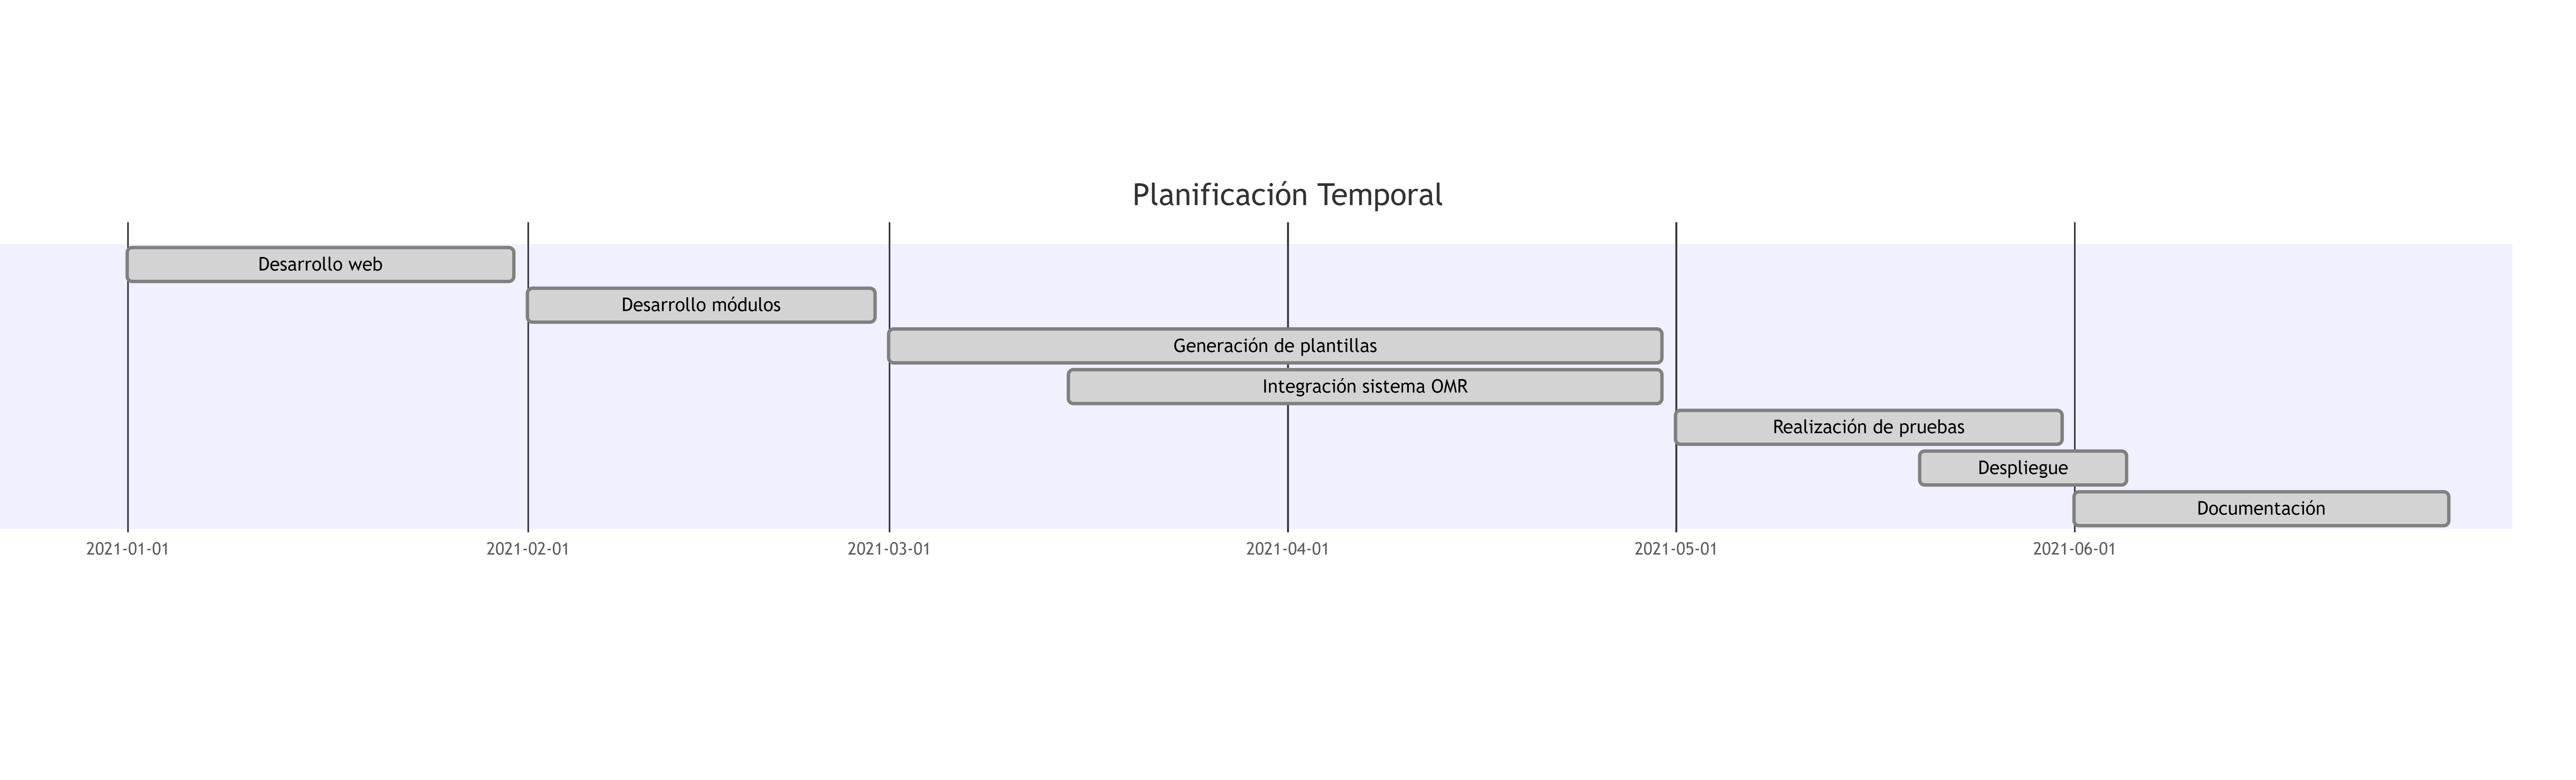
\includegraphics[width=15cm, height=6cm]{img/planificacion}
  \caption{Diagrama planificación temporal}
  \label{figura:planificacion}
\end{figure}

El mes de enero se dedicó al desarrollo de la página web. Una pequeña
aproximación fue alcanzada, con una interfaz básica de usuario que
contuviera todos aquellos elementos necesarios fijados en los requisitos
del sistema: sistema de usuarios, comportamiento responsivo, etc...

Febrero absorbió el mayor tiempo en el desarrollo de módulos genéricos
para la aplicación. El objetivo era el desarrollo de módulos desacoplados
del sistema que resolviesen
problemas específicos de implementación, como el acceso a ficheros
en el equipo y/o registros de eventos generados por la aplicación.

Los meses de marzo y abril fueron los más costosos. Se desarrolló el
sistema de generación de plantillas de la aplicación, se modificó el
sistema OMR utilizado para que encajase con nuestra solución y nuestros
requisitos, y finalmente se estableció la unión entre la aplicación web
y el sistema OMR.

Por último, el mes de mayo y junio estuvo dedicado a la realización de
pruebas y experimentos, mejorando así el rendimiento de la aplicación y 
corrigiendo problemas conocidos. Se estudió el sistema de despliegue para
su implementación y se desarrolló finalmente esta memoria.

La duración aproximada del proyecto ha sido de 6 meses, con una media
de 14 horas de dedicación semanales.



%%%%%%%%%%%%%%%%%%%%%%%%%%%%%%%%%%%%%%%%%%%%%%%%%%%%%%%%%%%%%%%%%%%%%%%%%%%%%%%%
%%%%%%%%%%%%%%%%%%%%%%%%%%%%%%%%%%%%%%%%%%%%%%%%%%%%%%%%%%%%%%%%%%%%%%%%%%%%%%%%
% ESTADO DEL ARTE %
%%%%%%%%%%%%%%%%%%%%%%%%%%%%%%%%%%%%%%%%%%%%%%%%%%%%%%%%%%%%%%%%%%%%%%%%%%%%%%%%

\cleardoublepage
\chapter{Estado del arte}
\label{chap:estado}

En este capítulo presentaremos las tecnologías utilizadas en este proyecto
y explicaremos el por qué de su elección.

\section{\textit{Python}} 
\label{sec:python}

Existen muchos lenguajes de programación en la actualidad. Todos ellos permiten
a los desarrolladores desarrollar aplicaciones para computadores.
\textit{Python}\footnote{\url{https://www.python.org/}} es uno de estos lenguajes.

Este lenguaje de programación es bastante popular a día de hoy, convirtiéndose
así en ser uno de los más utilizados en el mundo de la industria.
En la Figura~\ref{figura:lenguajes_programacion} se puede observar un
gráfico de los lenguajes de programación más aprendidos y buscados en
el año 2020.

Entre las características de \textit{Python} destaca la sencillez a la hora de
escribir el código de las
aplicaciones. Es un lenguaje considerado de alto nivel. Esto quiere decir
que permite al desarrollador abstraerse de problemáticas ya resultas, como
el acceso al sistema de ficheros del equipo, la gestión de la memoria, etc...
Esto permite que el desarrollo de aplicaciones sea bastante sencillo.
Además, la sencillez de escritura de código con este lenguaje hace que
existan muchas librerías ya desarrolladas para su utilización.
Por lo visto todo son ventajas al hablar de este increíble lenguaje. Sin
embargo, existe una problemática en su uso. \textit{Python} es un lenguaje
interpretado, es decir, el código escrito en este lenguaje no es compilado.
Esta característica propia del lenguaje provoca que la ejecución de los
programas sea más lenta comparada con programas desarrollados en lenguajes
compilados. En realidad, esta peculiaridad se hace más notoria al 
desarrollar aplicaciones que requieran poco tiempo de procesamiento.

\begin{figure}
  \centering
  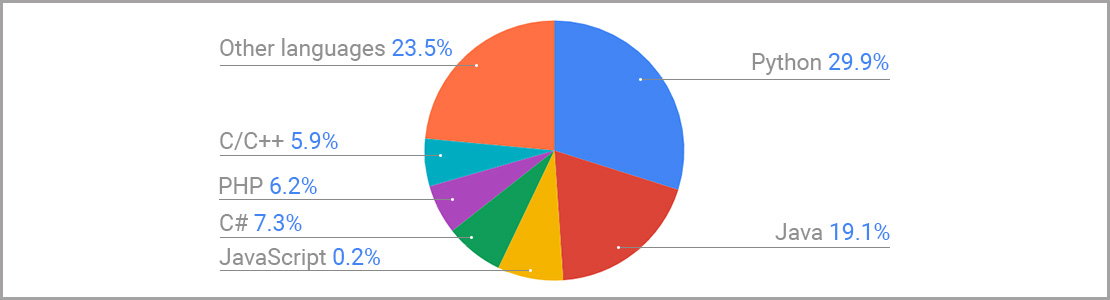
\includegraphics[width=12cm, keepaspectratio]{img/The-most-learned-languages}
  \caption{Lenguajes de programación más aprendidos en 2020. Fuente: scand.com}
  \label{figura:lenguajes_programacion}
\end{figure}

\textit{Python} dispone de una licencia \textit{Open source}\footnote{https://www.python.org/download/releases/3.4.2/license/}
libre y gratuita,
es decir, permite su uso, modificación y distribución.

Hemos escogido \textit{Python} como lenguaje de programación para nuestro proyecto
debido a todas estas razones.

\section{Tecnologías web: HTML, CSS, JavaScript} 
\label{sec:tecnologias_web}

Las tecnologías web nos permiten desarrollar páginas web con lenguajes de marcado,
con el objetivo de que los usuarios finales pueden visualizar correctamente
contenidos en estas páginas e interactuar con ellos.

Las tecnologías que se presentan en esta sección disponen de
licencias libres y gratuitas.

\subsection{HTML}
\label{subsec:html}

HTML (HyperText Markup Language) es un lenguaje de marcado de hipertexto.
Este lenguaje se utiliza desde el siglo veinte en la elaboración de páginas web.
Gracias a HTML podemos indicar la estructura de nuestro documento mediante
etiquetas, además de ofrecernos una gran adaptabilidad y estructura
lógica.

A lo largo de los años se han ido desarrollando diferentes versiones,
incorporando y suprimiendo diversas características. Esto ha permitido
que la tecnología poco a poco se convirtiera más eficiente y así
facilitar el desarrollo de páginas web a los desarrolladores.

El trabajo de HTML es definir la estructura de contenidos en una página web,
es decir, qué elementos se van a incluir y dónde se van a ubicar.

\subsection{CSS}
\label{subsec:css}

Cascading Style Sheets, más conocido como CSS, es un lenguaje de diseño
gráfico que nos permite definir la presentación de un lenguaje de marcado.
Una de sus aplicaciones es la presentación en páginas web, aunque tiene
más aplicaciones a día de hoy que no son tan conocidas.

La característica principal de esta tecnología es que se puede aplicar a
cualquier lenguaje de marcado, desacoplando contenido y forma totalmente.
Esto es una ventaja muy importante, ya que permite al desarrollador centrarse
exclusivamente en el alguno de estos aspectos (contenido o forma).

En nuestro proyecto esta tecnología es utilizada para definir la presentación
de los contenidos ofrecidos por HTML para nuestra página web.

\subsection{JavaScript}
\label{subsec:javascript}

Actualmente, todos los navegadores modernos soportan e interpretan el lenguaje
de programación conocido como JavaScript. El propósito de esta tecnología es
solucionar un problema latente en la presentación de páginas web al usuario final:
La interacción con la página web.

Como hemos comentado anteriormente, HTML nos permitía definir qué contenidos
aparecerían en nuestra página web final; CSS se ocupa de la presentación de 
esos contenidos; JavaScript por el contrario se ocupa de cómo el usuario interactúa
con esos contenidos, ofreciendo así una interfaz de usuario totalmente
dinámica.

JavaScript es un lenguaje muy utilizado a día de hoy, que tiene una gran
cantidad de aplicaciones prácticas. En este proyecto el lenguaje está
confinado en el desarrollo de tecnologías web.

\subsection{BootStrap}
\label{subsec:bootstrap}

BootStrap~\footnote{https://getbootstrap.com/} es un conjunto de librerías
CSS y JavaScript que facilitan el desarrollo de tecnologías web a los
desarrolladores.

Al utilizar estos \textit{plugins}, dotamos a nuestra página web de una interfaz
\textit{user-friendly}, creando aceptación en los usuarios finales.

En nuestro proyecto se utilizan las librerías BootStrap para aportar
a la página web un diseño responsivo y sencillo de utilizar.

\section{\textit{Django}} 
\label{sec:django}

\textit{Django}~\footnote{https://www.djangoproject.com/} ha sido utilizado en este
proyecto para crear la conexión entre el \textit{front end} y el
\textit{back end}. Es un \textit{framework} web para \textit{python} que permite el
desarrollo de tecnologías web de una manera fácil y rápida. Se encarga de
muchas de las complicaciones en el desarrollo web, tales como la gestión
de usuarios, el reconocimiento de \textit{urls}, para que el desarrollador
únicamente se centre es escribir su aplicación.

Entre las características de \textit{Django} destacan las siguiente:

\begin{itemize}
  \item Seguro: Evita errores comunes a la hora de desarrollar aplicaciones
  web. Su gestión de contraseñas mediante \textit{hashes} y la administración
  de usuarios permiten la protección del sitio web automáticamente.
  
  \item Mantenible: Una importante característica de \textit{Django} es que desacopla
  perfectamente partes del código para así resolver los problemas en un
  único sitio. Esto permite al desarrollador mantener de una forma bastante
  eficiente el código escrito.
  
  \item Portable: Al estar escrito en \textit{Python}, hace que sea soportado por
  muchas plataformas y distribuciones, como Linux, Windows, Mac OS X, etc.
\end{itemize}

Con respecto a la licencia de \textit{Django}, ésta corresponde a una licencia
\textit{Open source} libre y gratuita.

\section{\textit{Filepond}}
\label{sec:filepond}

\textit{Filepond}~\footnote{https://pqina.nl/filepond/} es una librería JavaScript
que permite la subida de documentos en páginas web de una forma sencilla
e intuitiva. Además, optimiza la subida de ficheros haciendo el proceso mucho más
rápido y seguro. Adicionalmente ofrece una alta accesibilidad y una
perfecta interfaz de usuario.

Es totalmente personalizable, permitiendo al desarrollador definir
el lenguaje en el que se muestran los
mensajes de información al usuario, el estilo de las cajas de subidas
de documentos, etc. En la Figura~\ref{figura:ejemplo_filepond} podemos ver un ejemplo de
caja para la subida de documentos con \textit{Filepond}.

\begin{figure}
  \centering
  
\includegraphics[width=5cm, keepaspectratio]{img/filepond_2}
  \caption{Ejemplo de subida de documentos con \textit{Filepond}}
  \label{figura:ejemplo_filepond}
\end{figure}

\textit{Filepond} posee una licencia MIT, la cual permite su uso, modificación
y/o distribución. Esta licencia, al igual que las anteriores, es libre y gratuita.

\section{\textit{Wkhtmltopdf}}
\label{sec:wkhtmltopdf}

Uno de los problemas a los que nos hemos enfrentado en este proyecto es
la generación de las plantillas de exámenes para los usuarios. Para el diseño
de estas plantillas se tomó la decisión de desarrollarlas en lenguaje HTML,
y posteriormente convertirlas a formato PDF. Para realizar esta conversión
se utilizó la herramienta \textit{Wkhtmltopdf}\footnote{https://wkhtmltopdf.org/}.

\textit{Wkhtmltopdf} es un conjunto de herramientas que permite al desarrollador
transformar documentos escritos
en formato HTML a documentos PDF.

Para la integración de esta herramienta con el sistema \textit{back end}
se utilizó un \textit{wrapper} para \textit{Python} llamado
\textit{Pdfkit}\footnote{https://pypi.org/project/pdfkit/}. Este módulo nos
permitió utilizar la funcionalidad proporcionada por \textit{Wkhtmltopdf} a través
del lenguaje \textit{Python}.

Con respecto a su licencia, \textit{Wkhtmltopdf} tiene una licencia
\textit{Gnu Lesser General Public}, la cual es libre y gratuita.

\section{\textit{Jinja2}}
\label{sec:jinja2}

\textit{Jinja2}\footnote{https://pypi.org/project/Jinja2/} es un módulo
de \textit{python} que permite la elaboración de documentos en texto
plano dinámicos. Posee una licencia \textit{BSD} de libre uso.

Esta herramienta nos ha permitido desarrollar las plantillas
de exámenes en lenguaje HTML de forma que se adaptasen a los criterios de
los usuarios: número de preguntas de examen, número de respuestas,
identificación del centro, etc. La documentación referente a \textit{Jinja2} está
accesible en \cite{jinja2:documentation}

\section{Sistema \textit{back end}} 
\label{sec:omr}

\begin{figure}
  \centering
  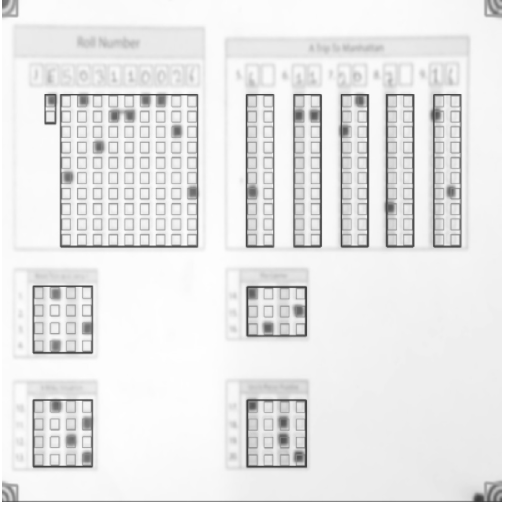
\includegraphics[width=7cm, keepaspectratio]{img/omr_1}
  \caption{El sistema OMR ubica las secciones del documento}
  \label{figura:uso_template_omr}
\end{figure}

La piedra angular de este proyecto es la tecnología OMR. El sistema utilizado
para el \textit{Back End} es un proyecto de código abierto con su correspondiente repositorio en
\textit{\textit{Github}}\footnote{https://github.com/Udayraj123/OMRChecker}.

El proyecto está desarrollado en \textit{python}, y nos da la facilidad de subir
documentos escaneados o fotografiados para que el sistema OMR detecte
automáticamente las marcas de tinta y corrija los exámenes.

El sistema ubica secciones previamente definidas en el documento aportado
tal y como se puede observar en la Figura~\ref{figura:uso_template_omr}.
Esto permite adaptarse a cualquier plantilla de examen tipo test.
Para ubicar estas secciones el sistema OMR entiende un determinado fichero
JSON\footnote{https://www.json.org/json-en.html} con una estructura
determinada, el cual el desarrollador debe modificar para que el sistema
se ajuste a su plantilla de una forma correcta.

Otra característica importante de este sistema es que es capaz de reconocer
las delimitaciones de un documento en una fotografía subida. Esto nos permite
realizar fotografías de nuestros documentos y automáticamente el sistema
nos lo reconocerá y lo alineará. Este funcionamiento se puede ver en la
Figura~\ref{figura:reconocimiento_doc_omr}.

\begin{figure}
  \centering
  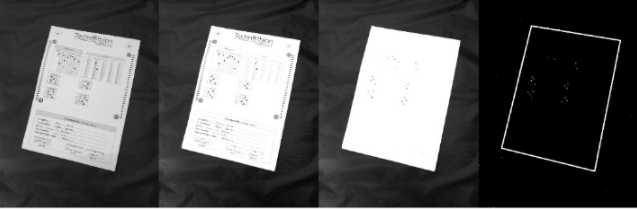
\includegraphics[width=10cm, keepaspectratio]{img/omr_2}
  \caption{El sistema OMR reconoce el documento subido}
  \label{figura:reconocimiento_doc_omr}
\end{figure}

Finalmente el sistema nos podrá devolver un documento \textit{.csv} con
las soluciones y la nota final de nuestros exámenes corregidos tal y como
se puede observar en la Figura~\ref{figura:soluciones_omr}.

El proyecto sigue siendo mantenido por su autor, mejorando la arquitectura
y funcionamiento del sistema. Además posee una licencia
\textit{Gnu Lesser General Public}, que permite su uso, modificación y
distribución.

Hemos escogido este sistema como \textit{Back End} debido a sus características
y correcto funcionamiento. Otros sistemas que se barajaron para este proyecto
fueron los siguientes:

\begin{itemize}
  \item https://github.com/rbaron/omr
  \item https://github.com/jansenfelipe/omr
  \item http://www.formscanner.org/
\end{itemize}

Uno de los inconvenientes de estos sistemas mencionados es que su desarrollo
ha sido abandonado. Por ejemplo, la aplicación \textit{formscanner} se detuvo
en 2017 y en Ubuntu 18.04 ya no funciona.
En segundo lugar, la mayoría de estos sistemas están basados en plantillas de
hojas de cálculo
y procesadores de texto, lo cuál dificulta su uso. Además, algunos dependen
de herramientas externas, como el caso de \textit{formscanner}, que depende
de \textit{XnConvert} \textit{Ghostscript} y la calidad del reconocimiento
no es buena.


\begin{figure}
  \centering
  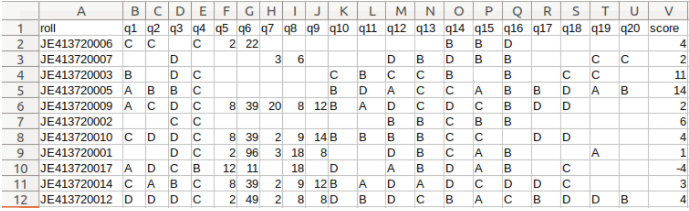
\includegraphics[width=10cm, keepaspectratio]{img/omr_3}
  \caption{El sistema OMR devuelve documento .csv con las soluciones}
  \label{figura:soluciones_omr}
\end{figure}

Por último, cabe destacar que el tutor de este proyecto tiene
experiencia en el uso de sistemas
OMR para la corrección de exámenes, concretamente con la
aplicación \textit{formscanner}. Es una herramienta con muchas
limitaciones, por lo que nuestro propósito ha sido
desarrollar una aplicación
de mayor calidad.

\section{\textit{Docker}} 
\label{sec:docker}

El uso de la virtualización en sistemas es muy popular hoy en día. Esta
tecnología permite crear representaciones, basadas en software, de una
entidad física como aplicaciones, servidores, almacenamiento virtuales,
etc. Existen muchas herramientas que dan la posibilidad de crear estos
entornos de virtualización. \textit{Docker}~\footnote{https://www.docker.com/} es
una de ellas.

En el contexto del proyecto, \textit{Docker} ha sido utilizado como herramienta
de despliegue de la aplicación. Esta herramienta nos permite virtualizar
en un contenedor toda nuestra aplicación, creando así un entorno virtual
inmutable a cambios externos.

Esta decisión conlleva muchas ventajas, ya que \textit{Docker} ofrece un sistema
Linux como entorno para nuestra aplicación. De esta forma, la aplicación
sigue su correcto funcionamiento sin verse influenciada por el sistema
operativo desde el que es ejecutada.

La comunidad \textit{Docker} pone a disposición del desarrollador un repositorio
llamado \textit{Docker Hub}~\footnote{https://hub.docker.com/}, en el cual
los desarrolladores tienen la posibilidad de subir sus propias imágenes
creadas. De esta forma, las imágenes están accesibles para todo el que
quiera hacer uso de ellas.

Con respecto a su licencia, \textit{Docker} utiliza una licencia
\textit{Apache License 2.0}\footnote{https://github.com/moby/moby/blob/master/LICENSE},
la cual es libre y gratuita.

\begin{comment}
Descripción de las tecnologías que utilizas en tu trabajo. 
Con dos o tres párrafos por cada tecnología, vale. 
Se supone que aquí viene todo lo que no has hecho tú.

Puedes citar libros, como el de Bonabeau et al., sobre procesos estigmérgicos~\cite{bonabeau:_swarm}. 
Me encantan los procesos estigmérgicos.
Deberías leer más sobre ellos.
Pero quizás no ahora, que tenemos que terminar la memoria para sacarnos por fin el título.
Nota que el \~ \ añade un espacio en blanco, pero no deja que exista un salto de línea. 
Imprescindible ponerlo para las citas.

Citar es importantísimo en textos científico-técnicos. 
Porque no partimos de cero.
Es más, partir de cero es de tontos; lo suyo es aprovecharse de lo ya existente para construir encima y hacer cosas más sofisticadas.
¿Dónde puedo encontrar textos científicos que referenciar?
Un buen sitio es Google Scholar\footnote{\url{http://scholar.google.com}}.
Por ejemplo, si buscas por ``stigmergy libre software'' para encontrar trabajo sobre software libre y el concepto de \emph{estigmergia} (¿te he comentado que me gusta el concepto de estigmergia ya?), encontrarás un artículo que escribí hace tiempo cuyo título es ``Self-organized development in libre software: a model based on the stigmergy concept''.
Si pulsas sobre las comillas dobles (entre la estrella y el ``citado por ...'', justo debajo del extracto del resumen del artículo, te saldrá una ventana emergente con cómo citar.
Abajo a la derecha, aparece un enlace BibTeX.
Púlsalo y encontrarás la referencia en formato BibTeX, tal que así:

{\footnotesize
\begin{verbatim}
@inproceedings{robles2005self,
  title={Self-organized development in libre software:
         a model based on the stigmergy concept},
  author={Robles, Gregorio and Merelo, Juan Juli\'an 
          and Gonz\'alez-Barahona, Jes\'us M.},
  booktitle={ProSim'05},
  year={2005}
}
\end{verbatim}
}

Copia el texto en BibTeX y pégalo en el fichero \texttt{memoria.bib}, que es donde están las referencias bibliográficas.
Para incluir la referencia en el texto de la memoria, deberás citarlo, como hemos hecho antes con~\cite{bonabeau:_swarm}, lo que pasa es que en vez de el identificador de la cita anterior (bonabeau:\_swarm), tendrás que poner el nuevo (robles2005self).
Compila el fichero \texttt{memoria.tex} (\texttt{pdflatex memoria.tex}), añade la bibliografía (\texttt{bibtex memoria.aux}) y vuelve a compilar \texttt{memoria.tex} (\texttt{pdflatex memoria.tex})\ldots y \emph{voilà} ¡tenemos una nueva cita~\cite{robles2005self}!

También existe la posibilidad de poner notas al pie de página, por ejemplo, una para indicarte que visite la página del GSyC\footnote{\url{http://gsyc.es}}.


Hemos hablado de cómo incluir figuras.
Pero no hemos dicho nada de tablas.
A mí me gustan las tablas.
Mucho.
Aquí un ejemplo de tabla, la Tabla~\ref{tabla:ejemplo} (siento ser pesado, pero nota cómo he puesto la referencia).

\begin{table}
 \begin{center}
  \begin{tabular}{ | l | c | r |} % tenemos tres colummnas, la primera alineada a la izquierda (l), la segunda al centro (c) y la tercera a la derecha (r). El | indica que entre las columnas habrá una línea separadora.
    \hline
    Uno & 2 & 3 \\ \hline % el hline nos da una línea vertical
    Cuatro & 5 & 6 \\ \hline
    Siete & 8 & 9 \\
    \hline
  \end{tabular}
  \label{tabla:ejemplo}
  \caption{Ejemplo de tabla. Aquí viene una pequeña descripción (el \emph{caption}) del contenido de la tabla. Si la tabla no es autoexplicativa, siempre viene bien aclararla aquí.}
 \end{center}
\end{table}
\end{comment}



%%%%%%%%%%%%%%%%%%%%%%%%%%%%%%%%%%%%%%%%%%%%%%%%%%%%%%%%%%%%%%%%%%%%%%%%%%%%%%%%
%%%%%%%%%%%%%%%%%%%%%%%%%%%%%%%%%%%%%%%%%%%%%%%%%%%%%%%%%%%%%%%%%%%%%%%%%%%%%%%%
% DISEÑO E IMPLEMENTACIÓN %
%%%%%%%%%%%%%%%%%%%%%%%%%%%%%%%%%%%%%%%%%%%%%%%%%%%%%%%%%%%%%%%%%%%%%%%%%%%%%%%%

\cleardoublepage
\chapter{Diseño e implementación}

En este capítulo detallaremos el diseño de nuestra arquitectura y
describiremos los distintos componentes que la componen, realizando
especial énfasis en el desarrollo, funcionamiento, y soluciones
propuestas en la aplicación.

Cabe destacar que la aplicación ha sido desarrollada con el objetivo de que
sea utilizada por un profesor, es decir, los estudiantes no deberían
relacionarse directamente con la aplicación.


\section{Arquitectura general} 
\label{sec:arquitectura}

La aplicación web ExChecker sigue la arquitectura cliente-servidor. Esto
quiere decir que los dos extremos de la comunicación estarán identificados.
El cliente realizará peticiones al servidor, y éste, a su vez, las resolverá,
devolviendo al cliente las respuestas a sus solicitudes.

Al ser nuestra aplicación una aplicación web, las solicitudes de los clientes
serán solicitudes a través del protocolo
HTTP~\footnote{https://en.wikipedia.org/wiki/Hypertext\_Transfer\_Protocol}.
Los navegadores web, tales
como Google Chrome, Mozila Firefox, Internet Explorer\dots se corresponden
a los clientes HTTP que manejan estas solicitudes, para posteriormente
renderizar las respuestas al usuario final.

Estas solicitudes llegarán a nuestro servidor HTTP, desarrollado con el
\textit{framework} de \textit{Python} \textit{Django}. El sistema, gracias a la información proporcionada
por el cliente, es capaz de resolver estas peticiones. Las peticiones
que el cliente puede realizar al servidor están definidas en la API de
comunicaciones (ver Anexo~\ref{app:api}).

En la figura~\ref{figura:arquitectura} podemos observar un diagrama
simplificado de nuestra arquitectura, simulando una petición del cliente.
Este diagrama muestra la resolución de las dos peticiones más importantes
en nuestro sistema: la generación de plantillas de exámenes y la corrección
de éstos.

La solicitud de generación de plantilla se apoya, como se comentó anteriormente
en la sección~\ref{sec:wkhtmltopdf}, en la herramienta \textit{Wkhtmltopdf}.
Mientras tanto, las solicitudes de correcciones de exámenes utilizan el
sistema OMR mencionado en la sección~\ref{sec:omr}.

\begin{figure}
  \centering
  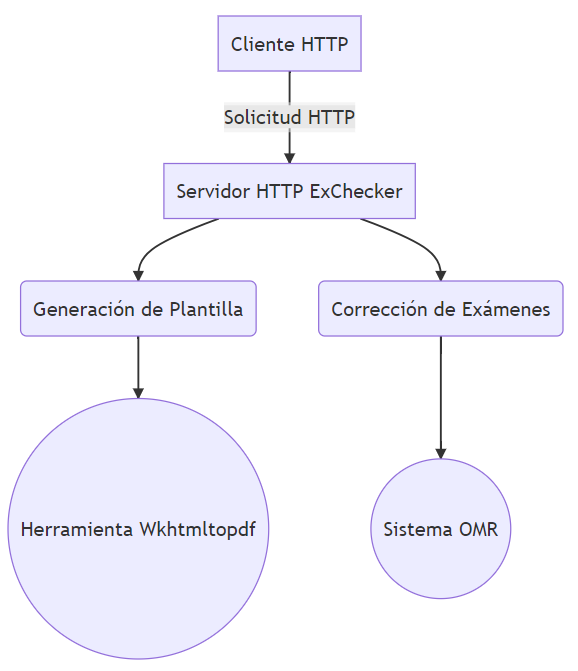
\includegraphics[width=10cm, keepaspectratio]{img/arquitectura}
  \caption{Arquitectura general del sistema}
  \label{figura:arquitectura}
\end{figure}

Finalmente, con el objetivo de presentar las siguientes secciones,
en la Figura~\ref{figura:pagina_principal} se muestra la página
principal de nuestra aplicación.
Esta página principal introduce al usuario en el uso de la aplicación,
indicándole dónde puede obtener las guías de usuario, cómo se generan
las plantillas, cómo corregir sus exámenes, etc.

\begin{figure}
  \centering
  
\includegraphics[width=12cm, keepaspectratio]{img/pagina_principal}
  \caption{Página principal de la aplicación}
  \label{figura:pagina_principal}
\end{figure}

\section{Sistema de usuarios}
\label{sec:sistema_usuarios}

Como comentábamos al inicio de esta memoria en la
sección~\ref{sec:objetivos-especificos}, la aplicación debe disponer
de un sistema de usuarios para así proporcionar la consistencia
independiente de datos.

Este sistema de usuarios ha sido implementado gracias al \textit{framework} \textit{Django},
que permite al desarrollador utilizar módulos ya generados para este fin.
La documentación sobre \textit{Django} utilizada en este proyecto puede consultarse
en \cite{django:documentation}.
Un usuario nuevo tiene la opción de registrarse en el sistema, introduciendo
un nombre de usuario por el cuál será identificado, nombre y apellidos.
Todos estos campos son
obligatorios para completar el registro. Una vez registrado, el usuario
tendrá acceso a funcionalidades adicionales en la aplicación. La página
de registro de usuarios se puede contemplar en la
Figura~\ref{figura:registro}

\begin{figure}
  \centering
  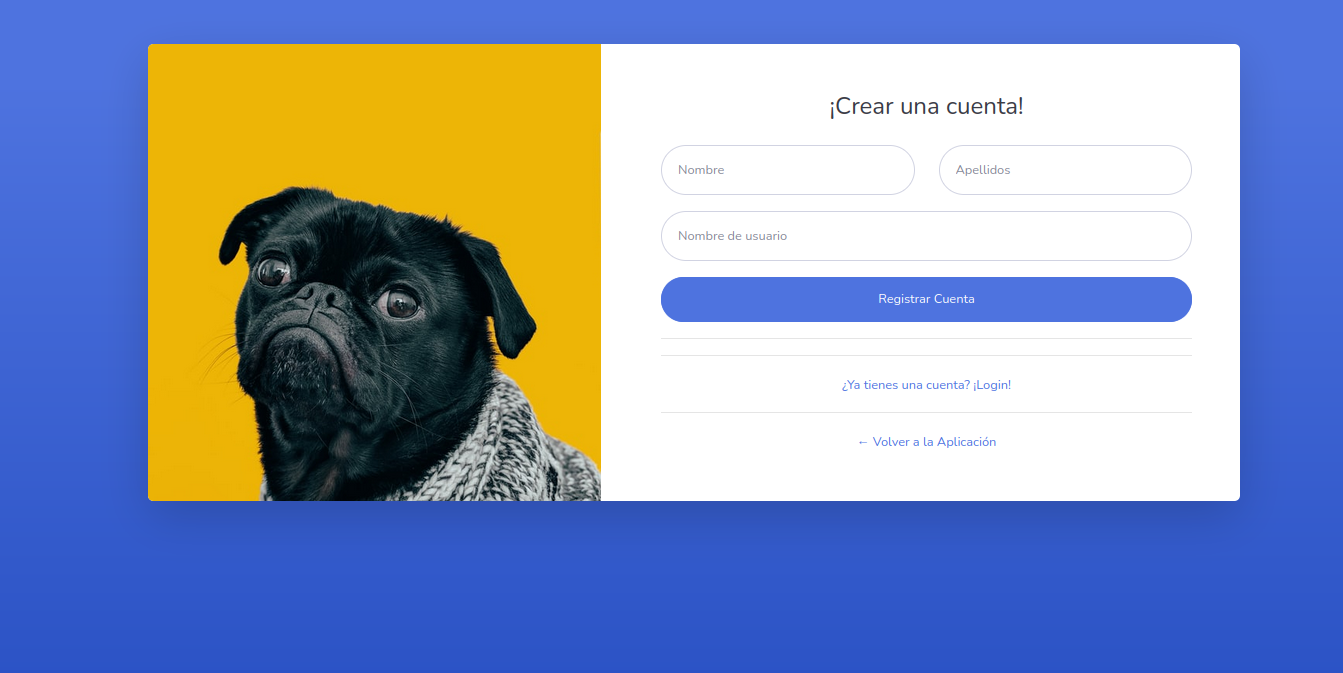
\includegraphics[width=12cm, keepaspectratio]{img/registro}
  \caption{Página de registro de usuarios}
  \label{figura:registro}
\end{figure}

ExChecker también proporciona la posibilidad de iniciar y cerrar la sesión
de usuario de una manera fácil y rápida. En la 
Figura~\ref{figura:login} se puede observar la página de inicio
de sesión de la aplicación. Es importante destacar que el sistema no utiliza
contraseñas para los usuarios. Esto es debido a que la aplicación está
desarrollada para ejecutarse en un entorno local, además de que no existe
información sensible que la aplicación guarde de los usuarios.

\begin{figure}
  \centering
  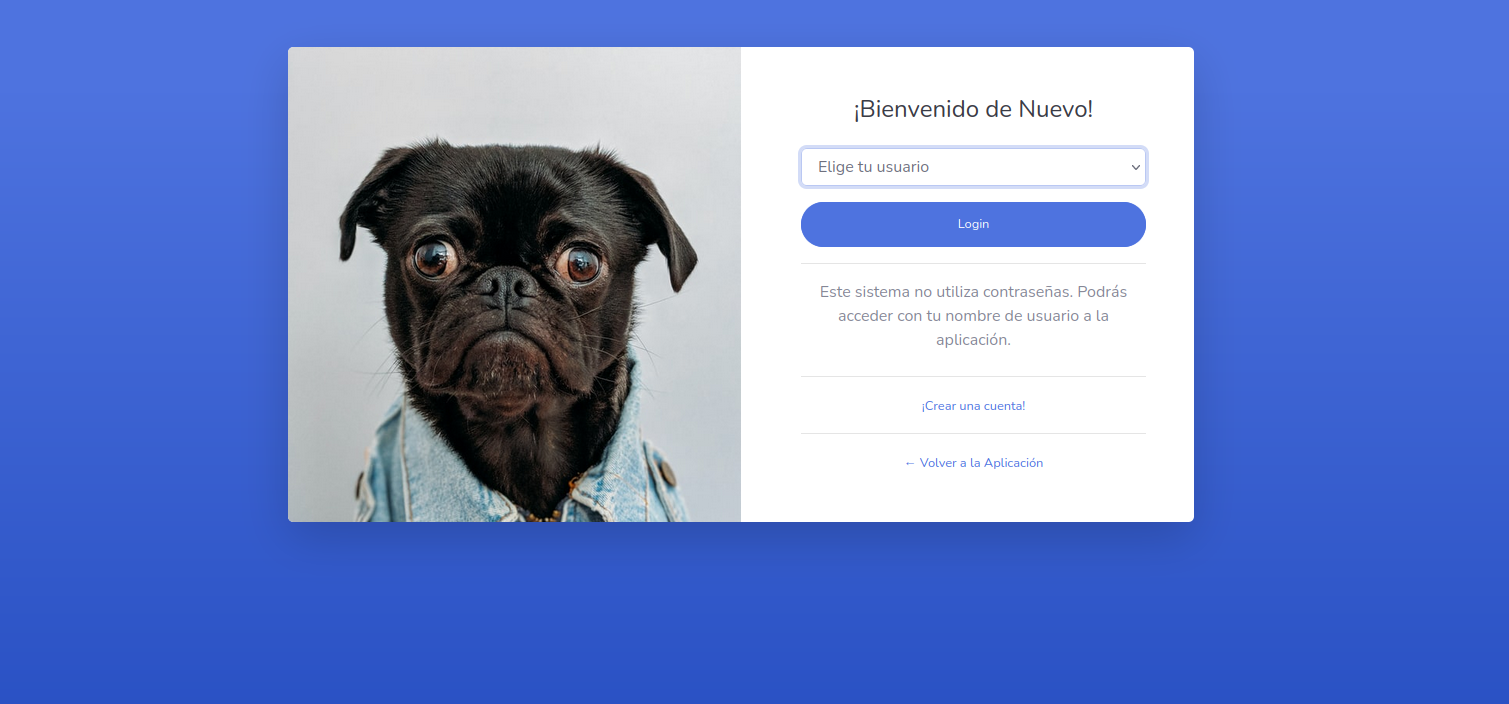
\includegraphics[width=12cm, keepaspectratio]{img/login}
  \caption{Página de inicio de sesión}
  \label{figura:login}
\end{figure}

\section{Generación de plantillas} 
\label{sec:generacion_plantillas}

La generación de plantillas ha sido una problemática bastante importante
en el desarrollo del proyecto. Como comentábamos en la 
sección~\ref{sec:objetivos-especificos}, el sistema de generación de
plantillas debe ser capaz de plasmar en un único documento PDF la
información que el usuario desea que aparezca en su plantilla. Esta
información se corresponde a la identificación del examen, identificación
del alumno, número de preguntas y número de respuestas por cada pregunta.
Esta información debe rellenarse en la página de generación de plantilla
de la aplicación, tal y como puede observarse en la
Figura~\ref{figura:generacion_plantilla}.

\begin{figure}
  \centering
  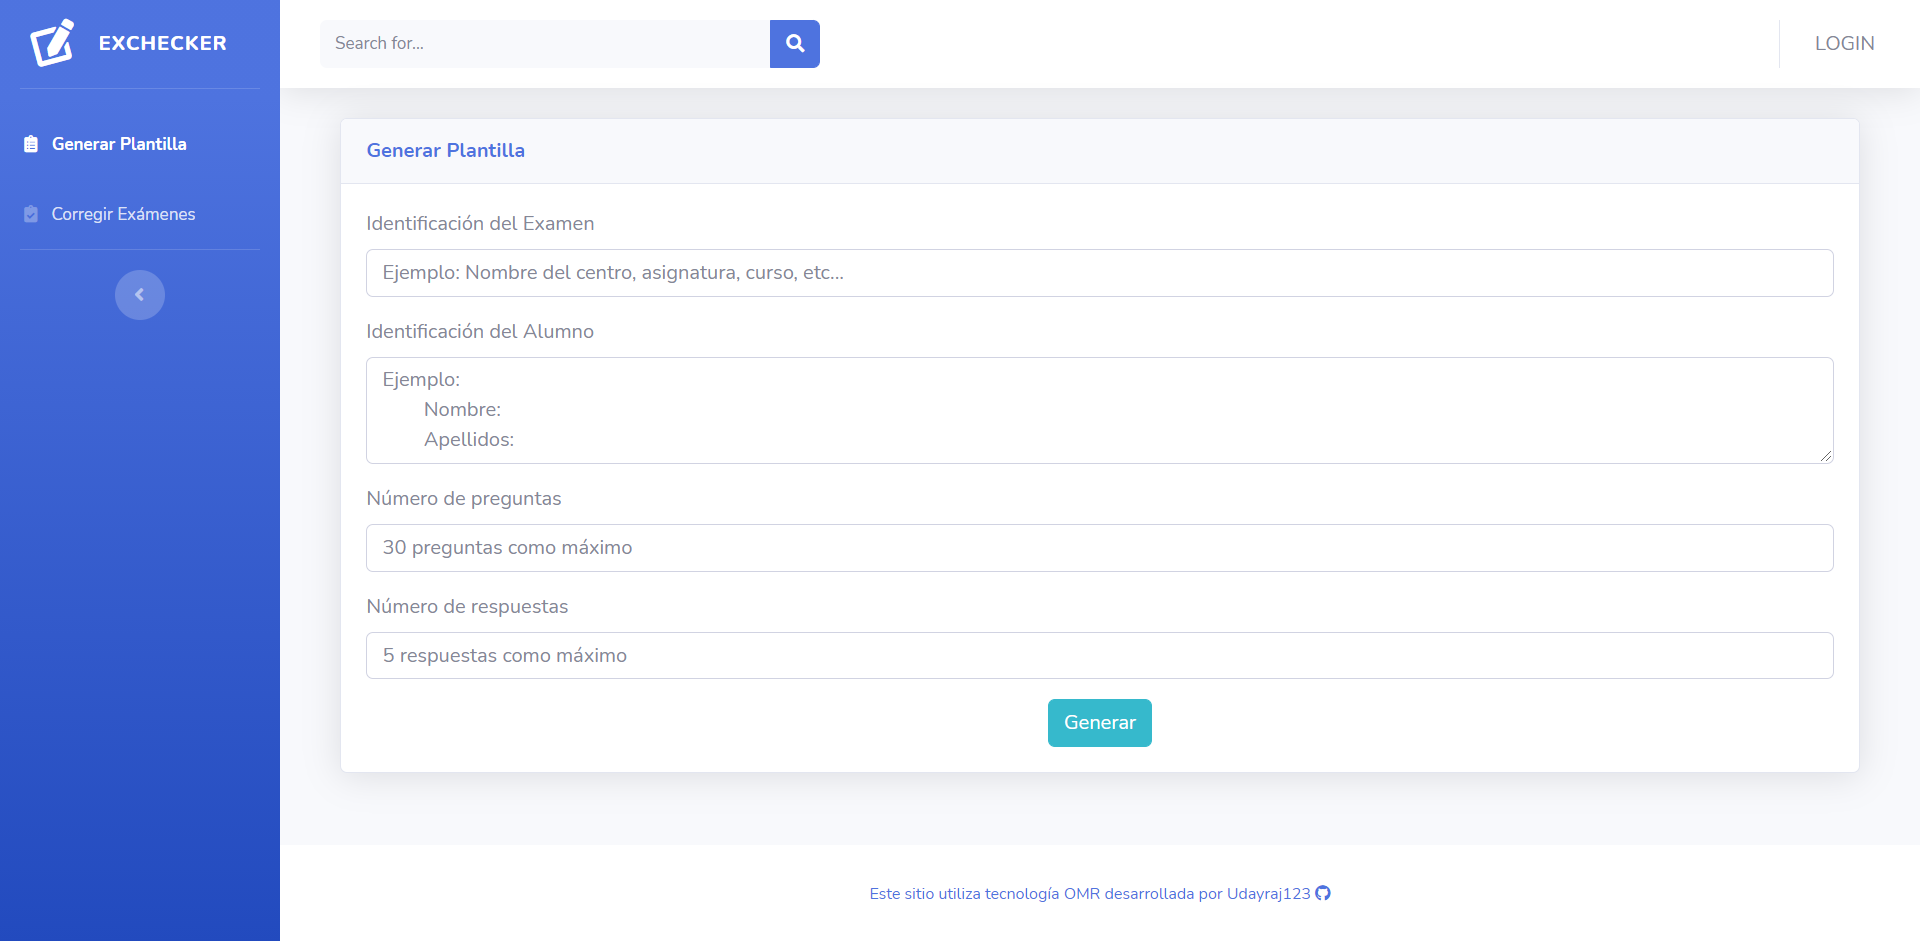
\includegraphics[width=12cm, keepaspectratio]{img/generacion_plantilla}
  \caption{Página de generación de plantilla}
  \label{figura:generacion_plantilla}
\end{figure}

Una vez realizada la petición de generación de plantilla, el sistema
genera un documento HTML renderizado con
\textit{Jinja2} pasando como parámetros
la información del usuario. La descripción de \textit{Jinja2} como tecnología utilizada
en este proyecto se ubica en la Sección~\ref{sec:jinja2}.
Finalmente se utiliza \textit{Wkhtmltopdf} para la 
conversión del documento HTML a documento PDF. Toda la documentación
sobre el uso de \textit{Wkhtmltopdf} y \textit{Pdfkit} puede encontrarse en
\cite{wkhtmltopdf:documentation, pdfkit:documentation}. En la
Figura~\ref{figura:ejemplo_plantilla} se muestra un ejemplo de
plantilla generada.

\begin{figure}
  \centering
  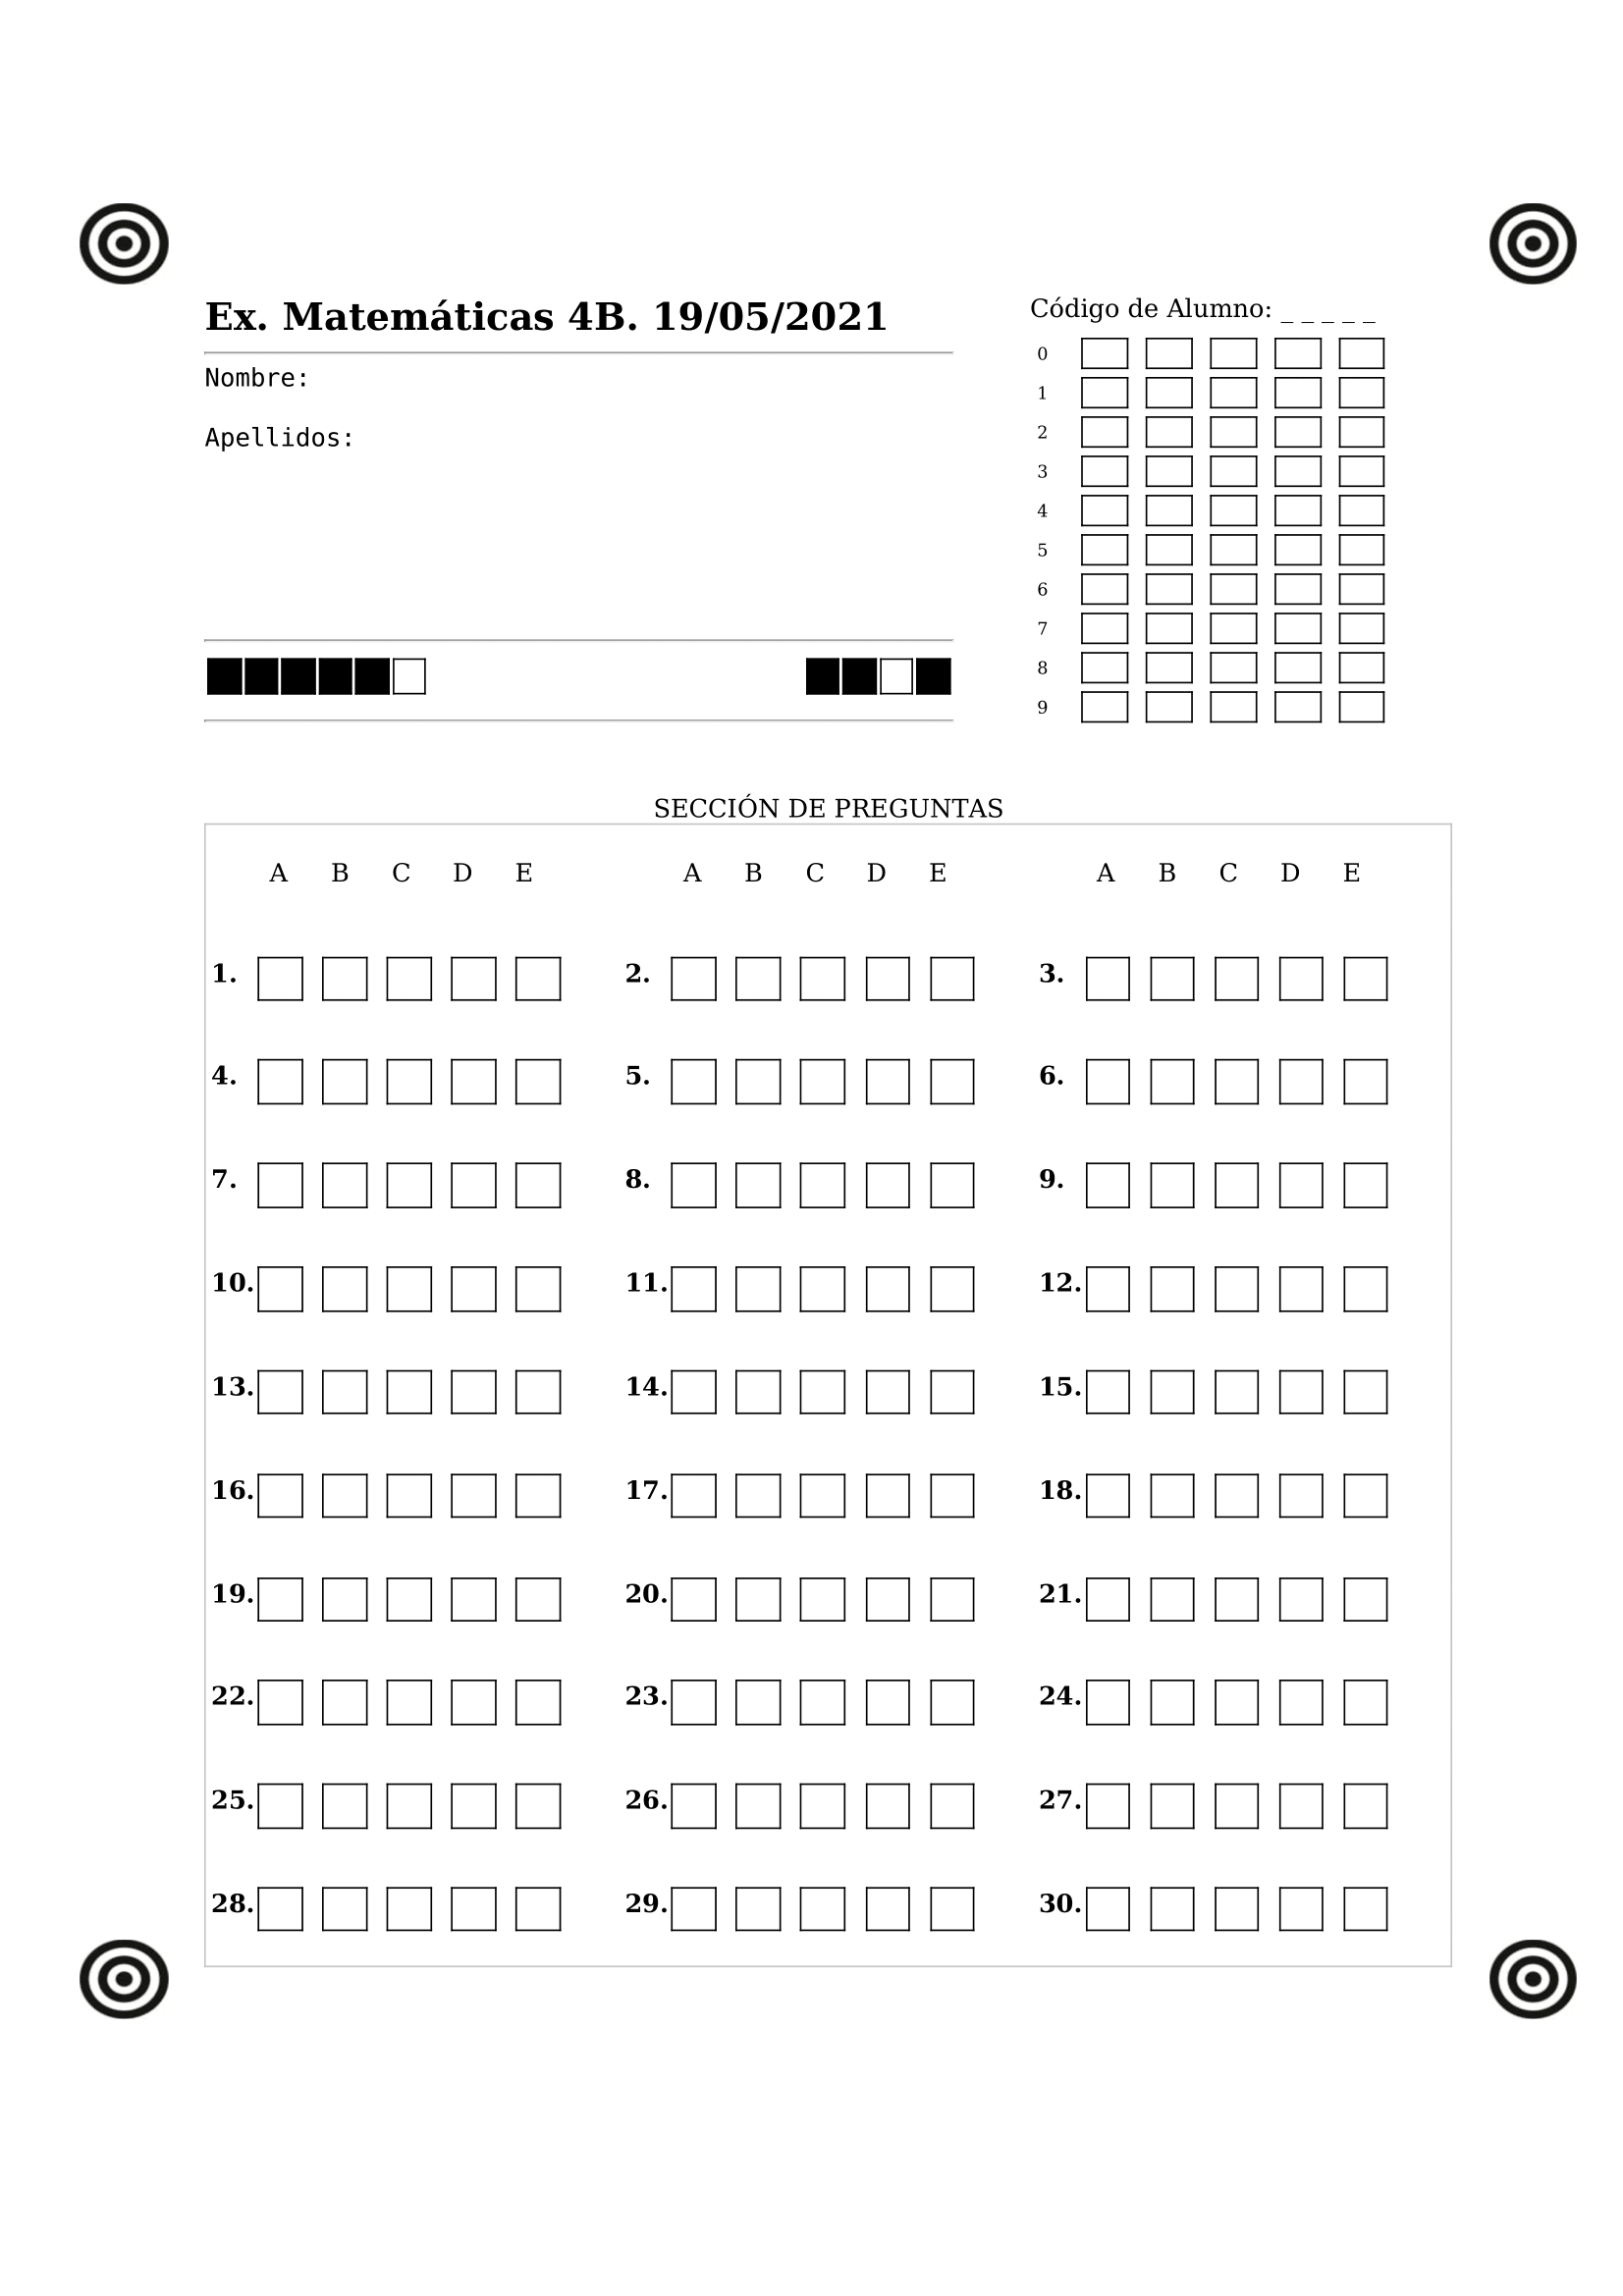
\includegraphics[width=9cm, keepaspectratio]{img/ejemplo_plantilla}
  \caption{Ejemplo de plantilla generada por ExChecker}
  \label{figura:ejemplo_plantilla}
\end{figure}

Las marcas que observamos en los vértices de la 
Figura~\ref{figura:ejemplo_plantilla} permiten al sistema OMR la
detección y alineación del documento. Además, el sistema añade una sección en la
plantilla generada llamada ``código de alumno''. En esta sección los alumnos
escribirán su código que permitirá identificarles en la corrección. Es importante
destacar que el examen con código de alumno 00000 será el documento que contendrá
las soluciones.

En el caso de que la generación de plantillas la realice un usuario \textit{logeado} en el
sistema, la plantilla generada se guardará junto a la fecha en la que se generó
la plantilla y un nombre
opcional que el usuario podrá aportar. De esta forma, el usuario podrá acceder a sus
plantillas guardadas con el objetivo de reutilizarlas en un futuro tal y como puede
observarse en la figura~\ref{figura:plantillas_usuario}

\begin{figure}
  \centering
  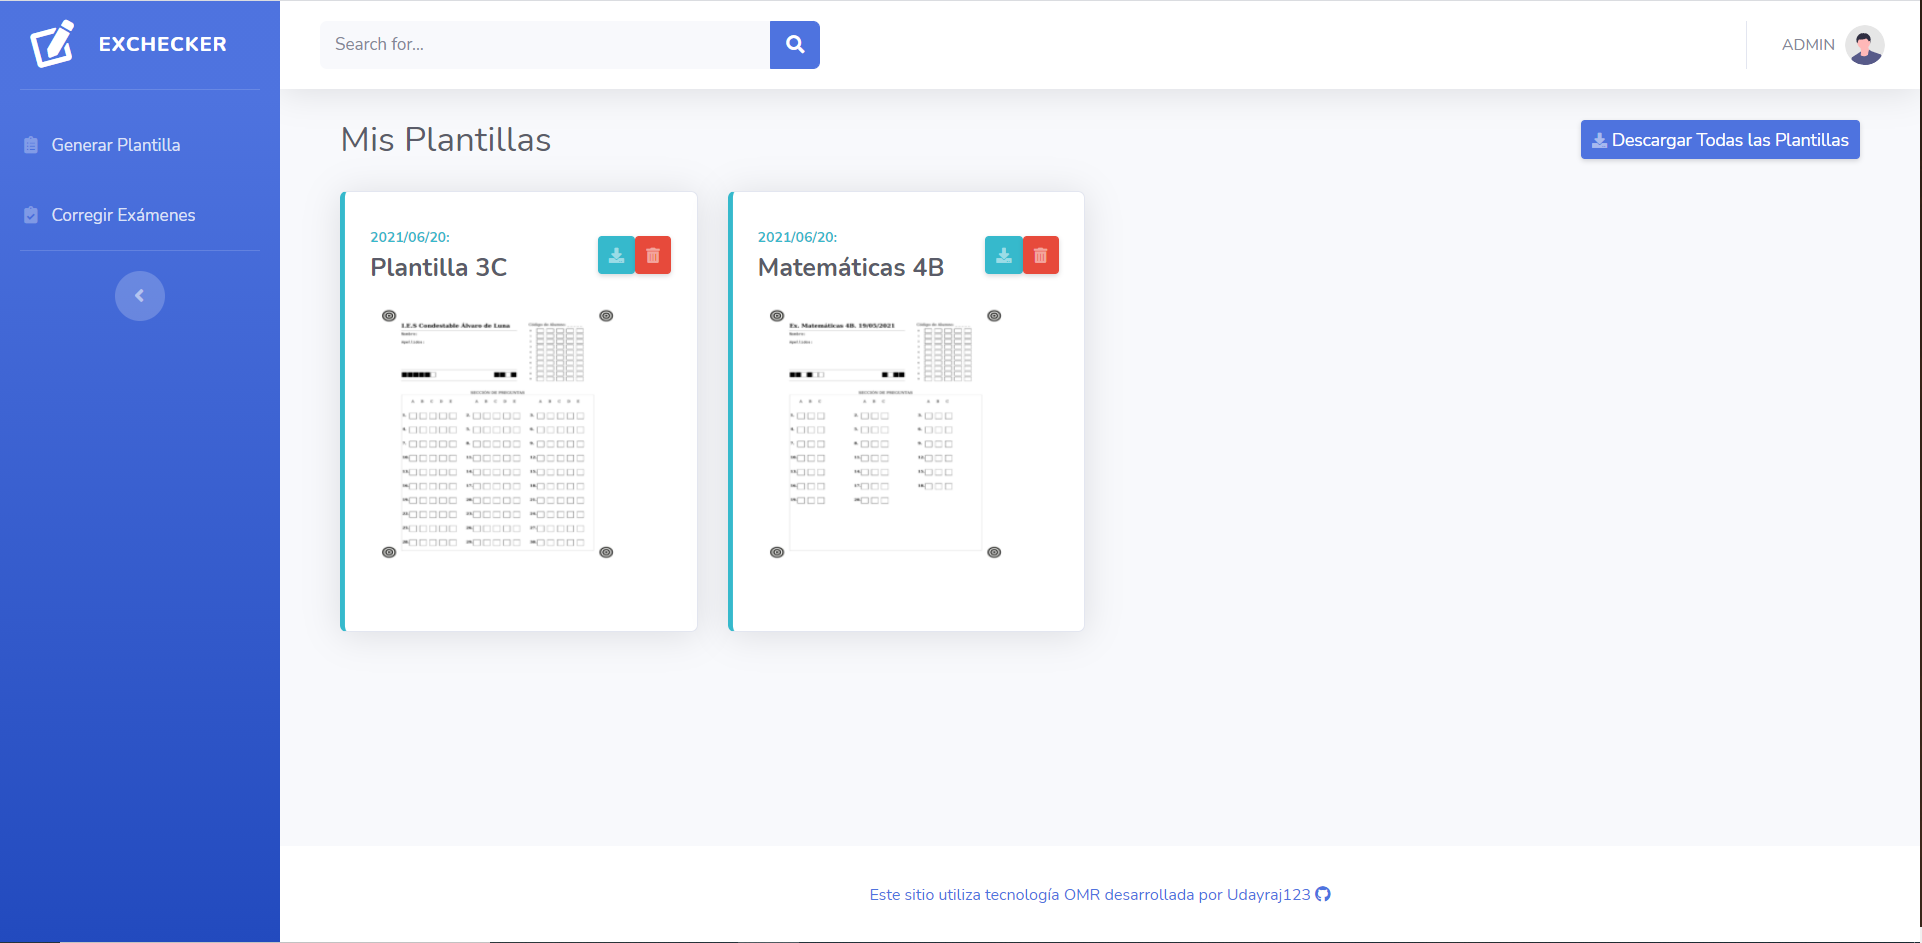
\includegraphics[width=12cm, keepaspectratio]{img/plantillas_usuario}
  \caption{Página de plantillas de usuario}
  \label{figura:plantillas_usuario}
\end{figure}

\subsection{Codificación del número de preguntas y respuestas}
\label{subsec:codificacion}

Al generarse la plantilla para los usuarios, el sistema incluye en ésta
campos auto rellenados que los alumnos no deberán rellenar.
Estos campos se utilizan para codificar el número de preguntas y respuestas
de la plantilla, tal y como se muestra en la
Figura~\ref{figura:codificaciones}.
De esta forma, cuando se suba la plantilla para su
corrección, el sistema entenderá estos campos y podrá extraer esta información
sin que el usuario tenga que indicarla nuevamente. El número de preguntas y respuestas
de la plantilla se codifica en notación binaria, por lo tanto, cada casilla
corresponde a un dígito binario: cero en el caso de estar la casilla vacía y uno
en el caso de estar rellenada. Además, cada codificación dispone de un bit de
paridad\footnote{Un bit de paridad es un dígito binario que indica si el
número de bits con un valor de 1 en un conjunto de bits es par o impar.}
que corresponde al bit más significativo. El objetivo de este bit es indicar
errores en la lectura de la plantilla. Por lo tanto, la codificación que aparece
en la Figura~\ref{figura:codificaciones} corresponde a una plantilla de 30
preguntas, ya que se observa el número binario 11110 (excluyendo el bit de paridad)
en su codificación, que corresponde al número 30 en el sistema decimal.
En cuanto al número de respuestas, la codificación nos muestra el número binario
101 (excluyendo el bit de paridad), que corresponde
al número 5 en el sistema decimal. Por lo tanto, la plantilla correspondiente
a esa codificación consta de
30 preguntas y 5 respuestas por pregunta.

\begin{figure}
  \centering
  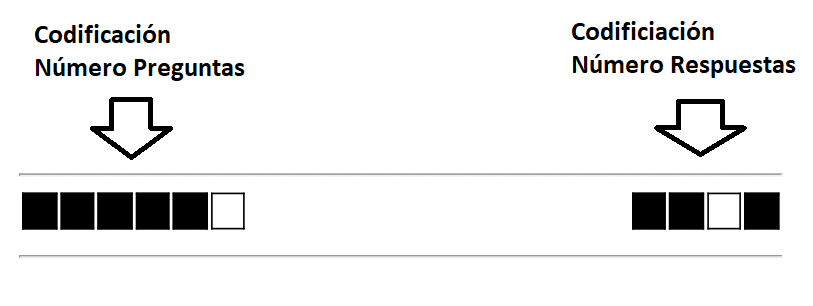
\includegraphics[width=10cm, keepaspectratio]{img/codificaciones}
  \caption{Codificación de número de preguntas y respuestas}
  \label{figura:codificaciones}
\end{figure}

\section{Corrección de exámenes} 
\label{sec:correccion_examenes}

Para la corrección de exámenes la aplicación dispone de una página destinada a tal
efecto. Esta página puede observarse en la Figura~\ref{figura:correccion_examenes}.
En ella el usuario tiene la posibilidad de indicar la nota máxima de los exámenes
y si el error en las respuestas penaliza. En el caso de que el usuario determine
que el error penalizará, se le permitirá el uso de la fórmula
tradicional\footnote{La fórmula tradicional indica que cada respuesta
incorrecta penalizará $\frac{1}{M}$ puntos a la nota final del examen,
siendo $M$ el número de respuestas por cada pregunta.} o indicar su propia penalización.

\begin{figure}
  \centering
  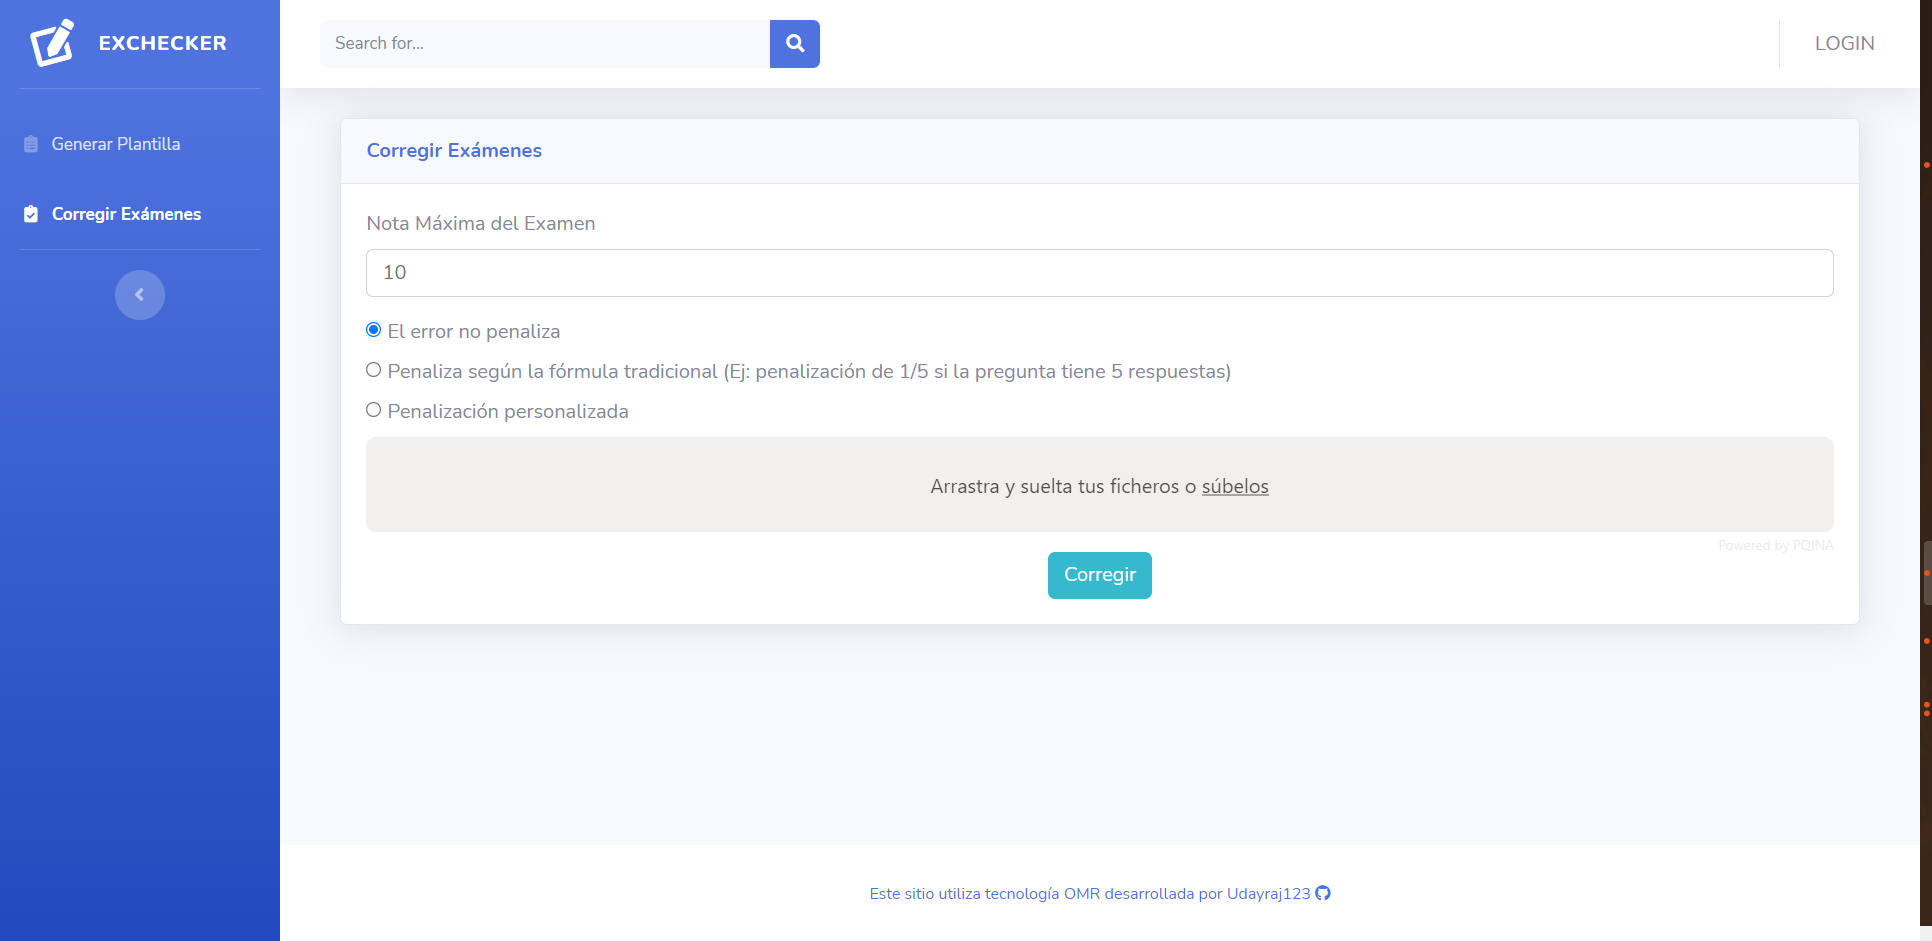
\includegraphics[width=12cm, keepaspectratio]{img/correccion_examenes}
  \caption{Página de corrección de exámenes}
  \label{figura:correccion_examenes}
\end{figure}

Es importante destacar que el sistema entiende el examen con código de alumno 00000
como el documento de respuestas. Esto quiere decir que para la corrección de
exámenes el sistema comparará las respuestas de cada examen con las respuestas
definidas en el documento de respuestas.
Esto se debe de tener en cuenta ya que será necesario
subir también este documento junto a todos los exámenes.

\subsection{Subida de ficheros}
\label{subsec:subida_ficheros}

Como comentábamos anteriormente en la Sección~\ref{sec:filepond}, la librería \textit{Filepond}
de JavaScript ha sido utiliza para facilitar la subida de ficheros por parte de los
usuarios. Toda la documentación referente a \textit{Filepond} puede
ser consultada en \cite{filepond:documentation}.
El funcionamiento de la subida de documentos es el siguiente:

\begin{enumerate}
  \item El usuario selecciona un documento de subida. En el momento de la selección,
  la librería \textit{Filepond} carga dinámicamente el documento y lo envía al sistema.
  \item El sistema reconoce el documento y genera un token\footnote{Número aleatorio
  que sirve de identificador.} que envía de vuelta a la librería \textit{Filepond}.
  \item La librería utiliza el token enviado por el sistema para identificar el documento
  subido. De esta forma, cualquier modificación que se realice al documento (por ejemplo
  descartarlo en la subida) se le comunicará al sistema utilizando este token.
  \item Finalmente, cuando el usuario confirma la subida de ficheros, \textit{Filepond} envía
  al sistema un lista de identificadores de documentos que el usuario ha aceptado.
  De esta forma, el sistema entiende que el usuario reconoce y acepta la subida de
  esos ficheros.
\end{enumerate}

La librería \textit{Filepond} es muy flexible, y permite al desarrollador elegir una lista de
\textit{plugins} que determinarán el comportamiento de la subida de ficheros. En este proyecto,
la subida de ficheros se ha limitado a 50 ficheros como máximo y los formatos de
documentos admitidos son .png, .jpg, .pdf. Además, se ha modificado la interfaz con
el usuario para admitir el idioma español.

Adicionalmente, el sistema verifica los documentos subidos, y en el caso de obtener
documentos en formato PDF convierte todas sus páginas en documentos en formato
PNG.

En la Figura~\ref{figura:subida_documentos} se puede apreciar un ejemplo de subida de documentos
en varios formatos.

\begin{figure}
  \centering
  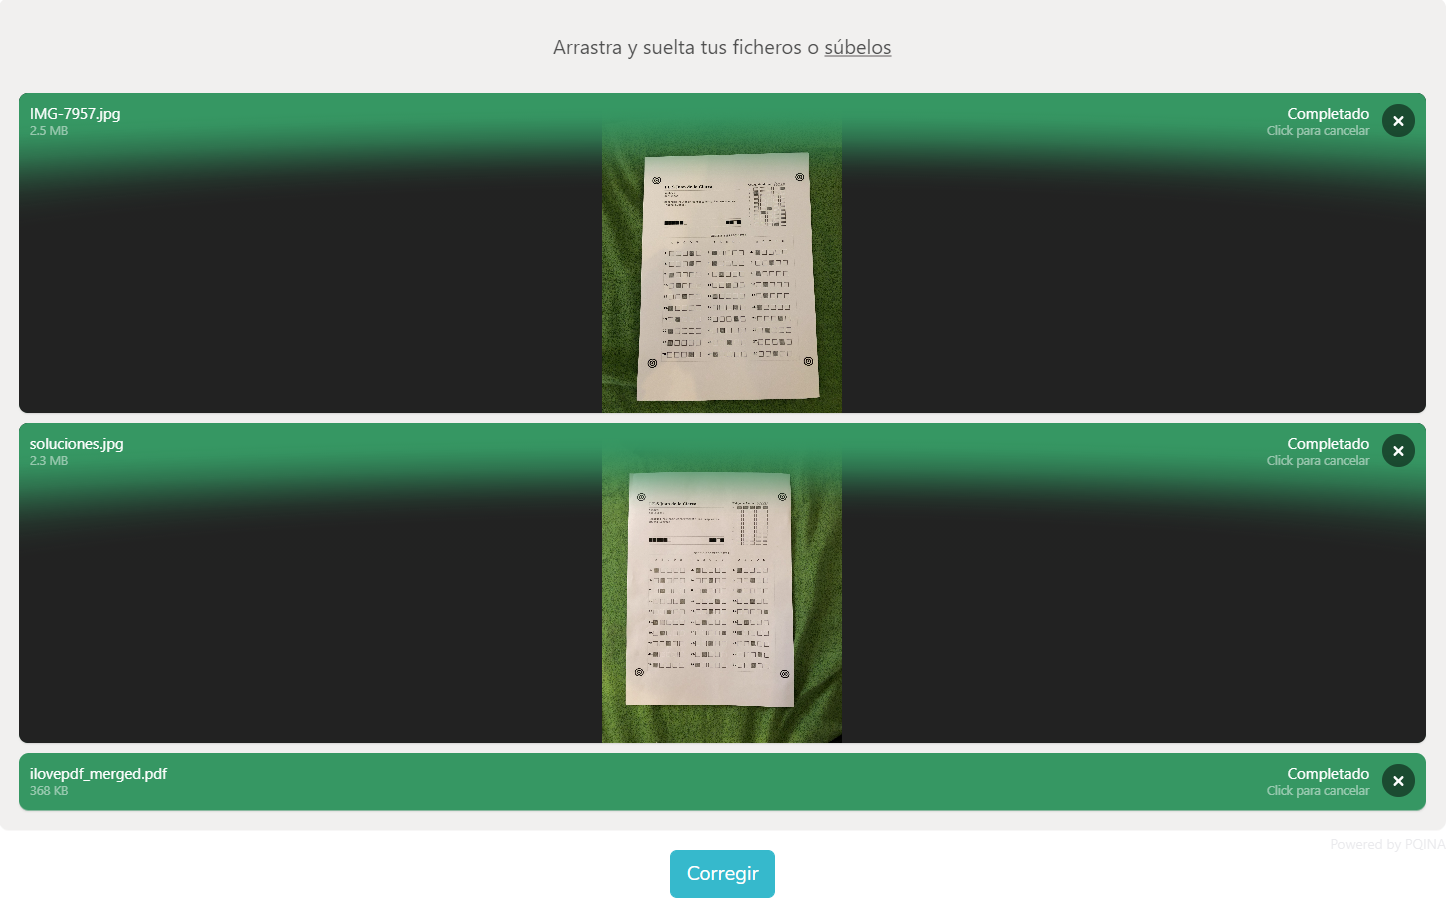
\includegraphics[width=12cm, keepaspectratio]{img/subida_documentos}
  \caption{Ejemplo de subida de documentos}
  \label{figura:subida_documentos}
\end{figure}

\subsection{Proceso de corrección}
\label{subsec:proceso_correccion}

Una vez subidos los documentos, el sistema los guardará y ejecutará el sistema OMR,
pasándole como parámetros la ruta en el sistema de ficheros donde se han guardado
los documentos. Es en este momento en el que el sistema OMR obtiene la información
de secciones de cada documento a partir del fichero JSON de configuración configurado
anteriormente (ver Sección~\ref{sec:omr}). En este fichero se detallan los campos
que el sistema OMR debe tener en cuenta para la corrección del examen. El fichero
utilizado para reconocer las secciones de las plantillas generadas por ExChecker
se indica en el Anexo~\ref{app:template_json}.

Finalmente, el sistema OMR detecta el documento en cuestión y aplica técnicas basadas
en filtros de imagen para detectar cambios significativos en las secciones de respuestas
indicadas en el fichero JSON. La decisión que toma el sistema para determinar si un campo está rellenado
o no se basa en un \textit{threshold} configurable. El resultado de este proceso
se puede observar en la Figura~\ref{figura:deteccion_respuestas}. Por último, el sistema OMR genera un
documento CSV con el valor de las respuestas detectadas en todos los exámenes.

\begin{figure}
  \centering
  \subfloat[Detección de respuestas]{
  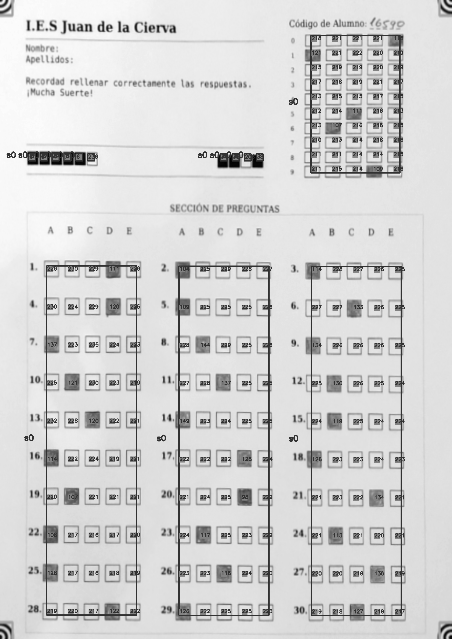
\includegraphics[width=7cm, height=10cm]{img/deteccion_respuestas1} }
  \subfloat[Detección de valores]{
  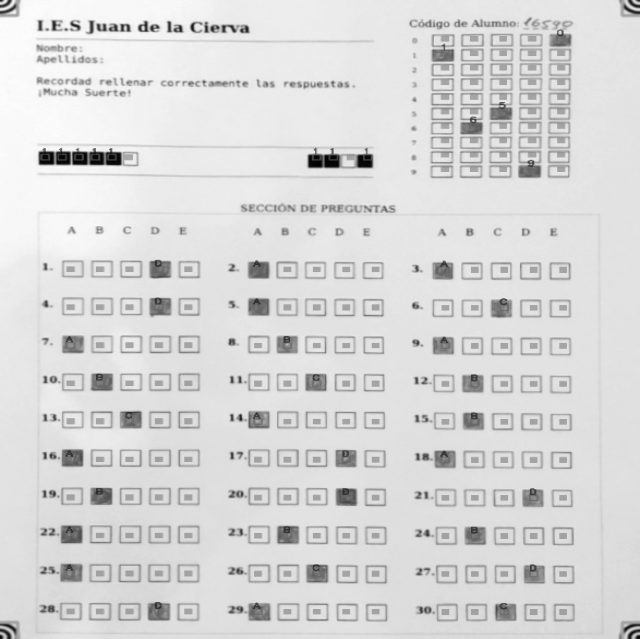
\includegraphics[width=7cm, height=10cm]{img/deteccion_respuestas2} }
  \caption{El sistema OMR detecta las respuestas de los exámenes}
  \label{figura:deteccion_respuestas}
\end{figure}

\subsection{Generación de resultados y estadísticas}
\label{subsec:estadisticas}

Una vez que el sistema OMR ha detectado todas las respuestas de los documentos subidos
y ha generado un documento CSV el sistema está en disposición
de analizar esa información. A continuación, se detalla el proceso de generación de
resultados y estadísticas gracias a la información proporcionada por el sistema OMR:

\begin{enumerate}
  \item En primer lugar, analizamos los valores obtenidos en busca de errores. Para ello
  comprobamos que no existan códigos de alumnos repetidos, que todos los bits de 
  paridad coincidan con su codificación, que el documento soluciones exista y y no
  tenga preguntas con respuestas múltiples, etc. En el caso de encontrar alguna
  anomalía se procederá a notificar al usuario y abortar la corrección
  (ver Subsección~\ref{subsec:correcciones_fallidas}).
  \item Una vez validadas las respuestas de cada examen, se procede a calcular la nota
  de cada alumno. Para ello, se compara cada respuesta con la respuesta correspondiente
  en el documento de soluciones. Para el cálculo de la nota final se tiene en cuenta
  los valores aportados por el usuario: nota máxima del examen y penalización por
  respuesta fallida. Finalmente se genera un nuevo documento CSV con las respuestas
  de cada alumno y la nota final de cada examen.
  \item Además, se analizan las respuestas de los alumnos y las notas finales
  con el objetivo de generar estadísticas informativas para el usuario: porcentaje
  de aprobados, porcentaje de suspensos, porcentaje de alumnos con respuestas en
  blanco, etc.
  \item Por último, se renderiza toda la información en una página HTML para que
  el usuario tenga la posibilidad de visualizar las estadísticas de la corrección
  y pueda descargarse el documento CSV con las respuestas y notas de cada alumno.
  En la Figura~\ref{figura:resultados_y_estadisticas} se puede observar
  un ejemplo de información mostrada
  en la finalización de la corrección de exámenes.
\end{enumerate}

\begin{figure}
  \centering
  \subfloat[Resultados y estadísticas 1]{
  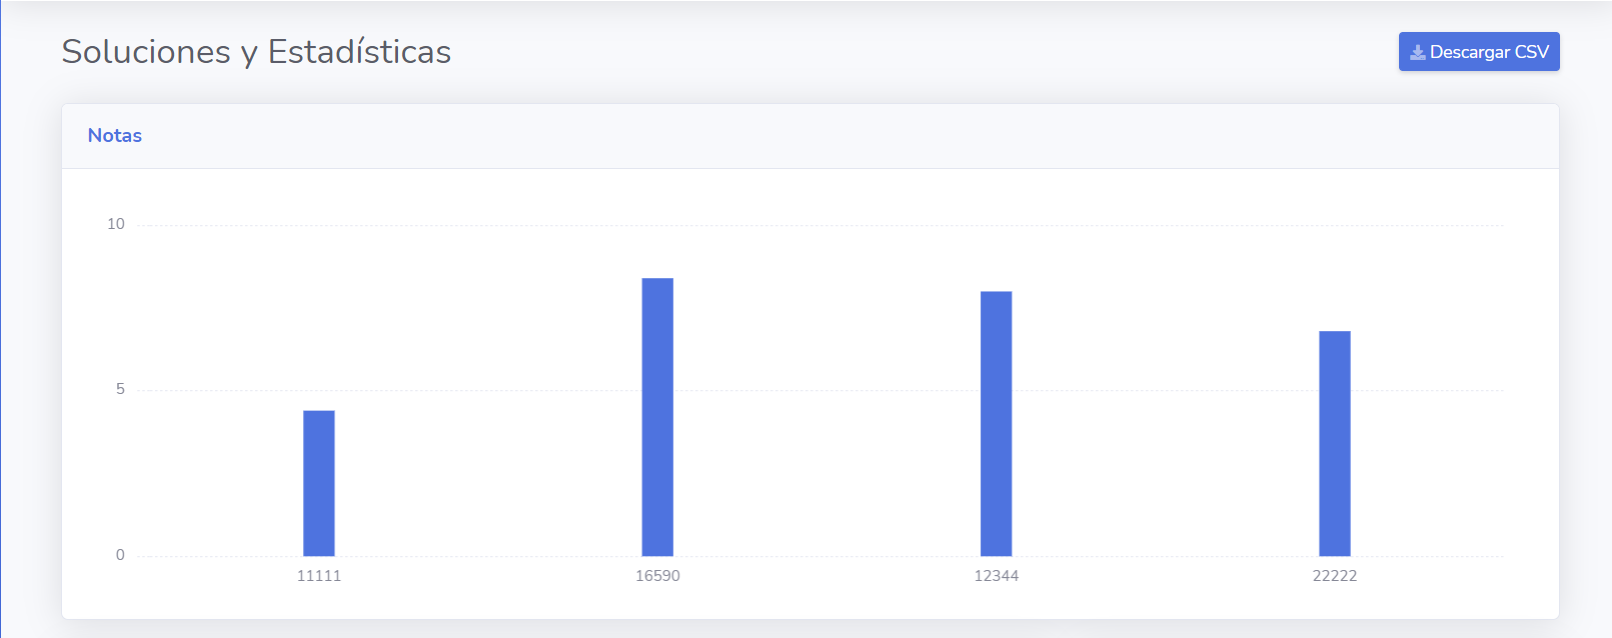
\includegraphics[width=5cm, height=3cm]{img/resultados_y_estadisticas1} }
  \subfloat[Resultados y estadísticas 2]{
  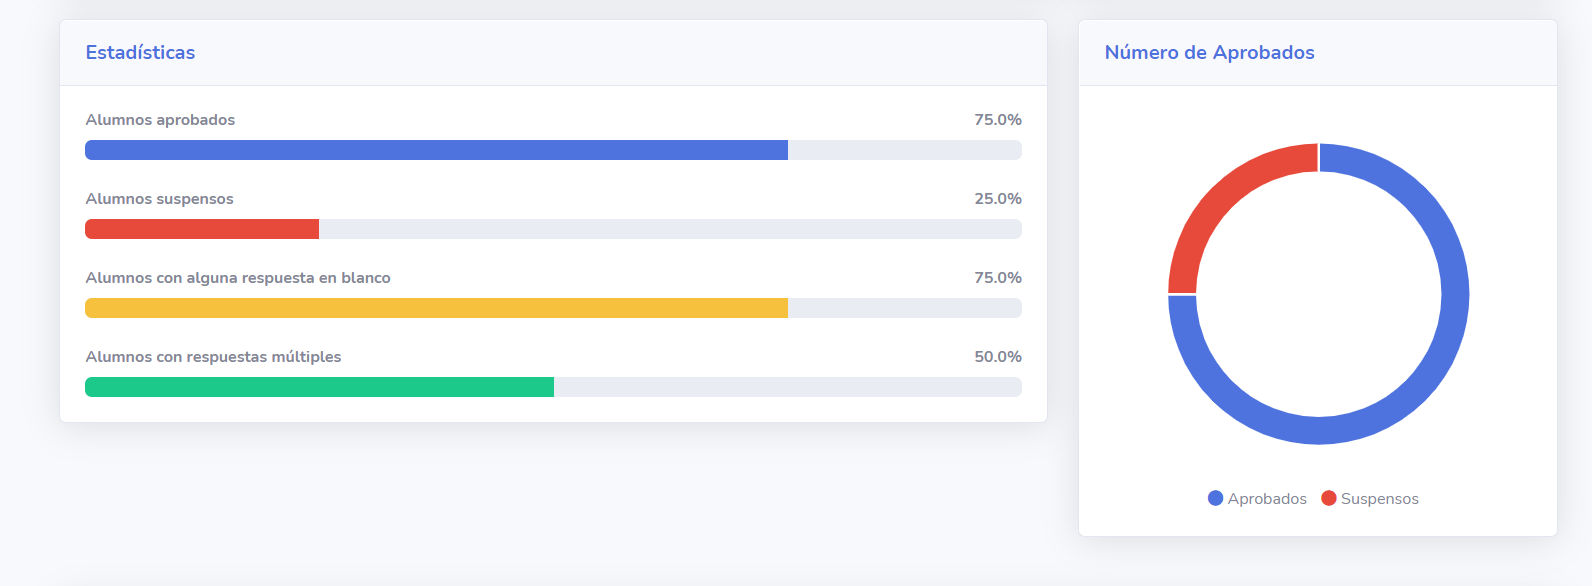
\includegraphics[width=5cm, height=3cm]{img/resultados_y_estadisticas2} }
  \subfloat[Resultados y estadísticas 3]{
  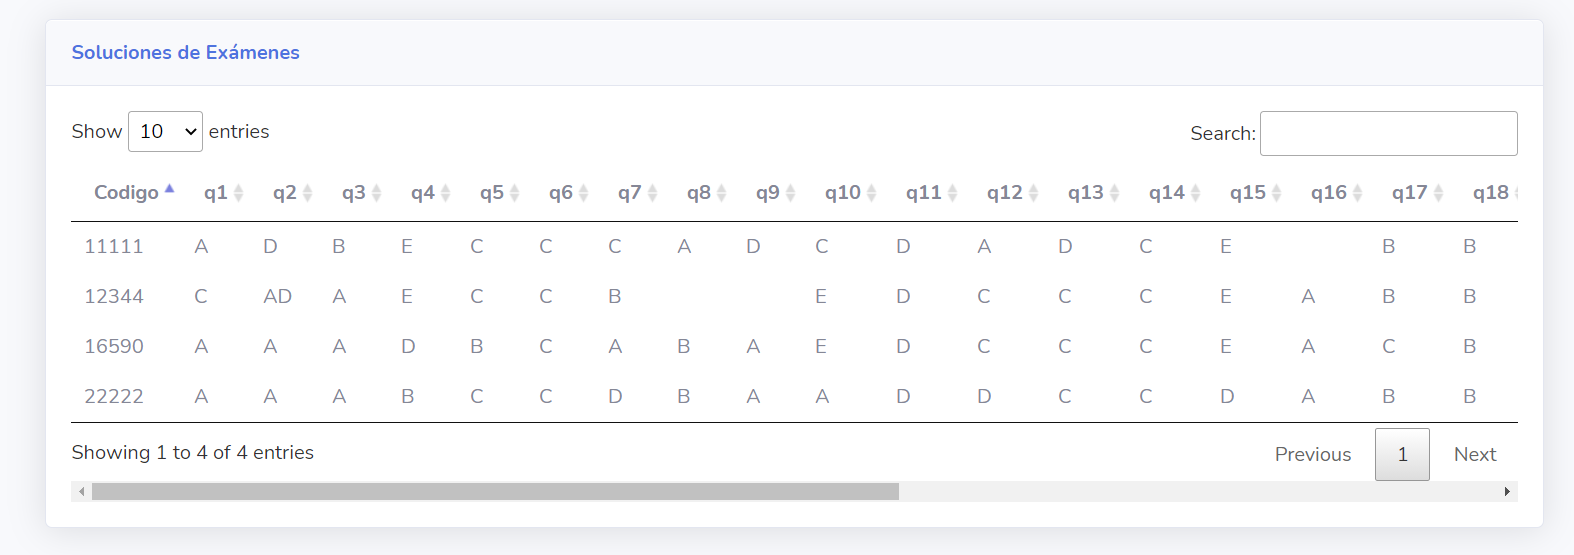
\includegraphics[width=5cm, height=3cm]{img/resultados_y_estadisticas3} }
  \caption{Página de resultados y estadísticas}
  \label{figura:resultados_y_estadisticas}
\end{figure}

\subsection{Correcciones fallidas}
\label{subsec:correcciones_fallidas}

Es posible que el usuario desee corregir un grupo de exámenes en los que exista
algún error: falta de documento de soluciones, repetición en algún código de alumno,
plantilla mal alineada, etc.

En la Tabla~\ref{tabla:errores} se indican los errores posibles que se pueden dar en la corrección
de exámenes y qué actuaciones toma el sistema ante éstos.

En la Figura~\ref{figura:error_en_correccion} se observa la página de error
a la que se le redirige al usuario
debido a algún error en la corrección de sus documentos.

\begin{table}[h]
  \begin{center}
    \begin{tabular}{ | p{7cm} | p{7cm} |}
      \hline
      \multicolumn{2}{|c|}{\textbf{Errores en corrección de exámenes}} \\
      \hline
      \centering \textbf{Error} & \centering \textbf{Actuación} \tabularnewline
      \hline
      \centering No se encuentra el documento soluciones &
      \centering Se notifica al usuario y se aborta la corrección \tabularnewline
      \hline
      \centering Únicamente se encuentra el documento soluciones &
      \centering Se notifica al usuario y se aborta la corrección \tabularnewline
      \hline
      \centering El documento soluciones presenta múltiples respuestas &
      \centering Se notifica al usuario y se aborta la corrección \tabularnewline
      \hline
      \centering Existe algún documento cuyo bit de paridad de codificación no coincide &
      \centering Se notifica al usuario y se aborta la corrección \tabularnewline
      \hline
      \centering Existen documentos con números de preguntas y respuestas distintas &
      \centering Se notifica al usuario y se aborta la corrección \tabularnewline
      \hline
      \centering Existen documentos con códigos de alumnos repetidos &
      \centering Se notifica al usuario y se aborta la corrección \tabularnewline
      \hline
      \centering Existen documentos con códigos de alumnos vacíos &
      \centering Se notifica al usuario y se aborta la corrección \tabularnewline
      \hline
      \centering Existen documentos con múltiples respuestas &
      \centering La pregunta en cuestión se determina no válida y se sigue con la corrección \tabularnewline
      \hline
      \centering Existen documentos con respuestas vacías &
      \centering La pregunta en cuestión se determina no válida y se sigue con la corrección \tabularnewline
      \hline
    \end{tabular}
    \caption{Errores en corrección de exámenes}
    \label{tabla:errores}
  \end{center}
\end{table}

\begin{figure}
  \centering
  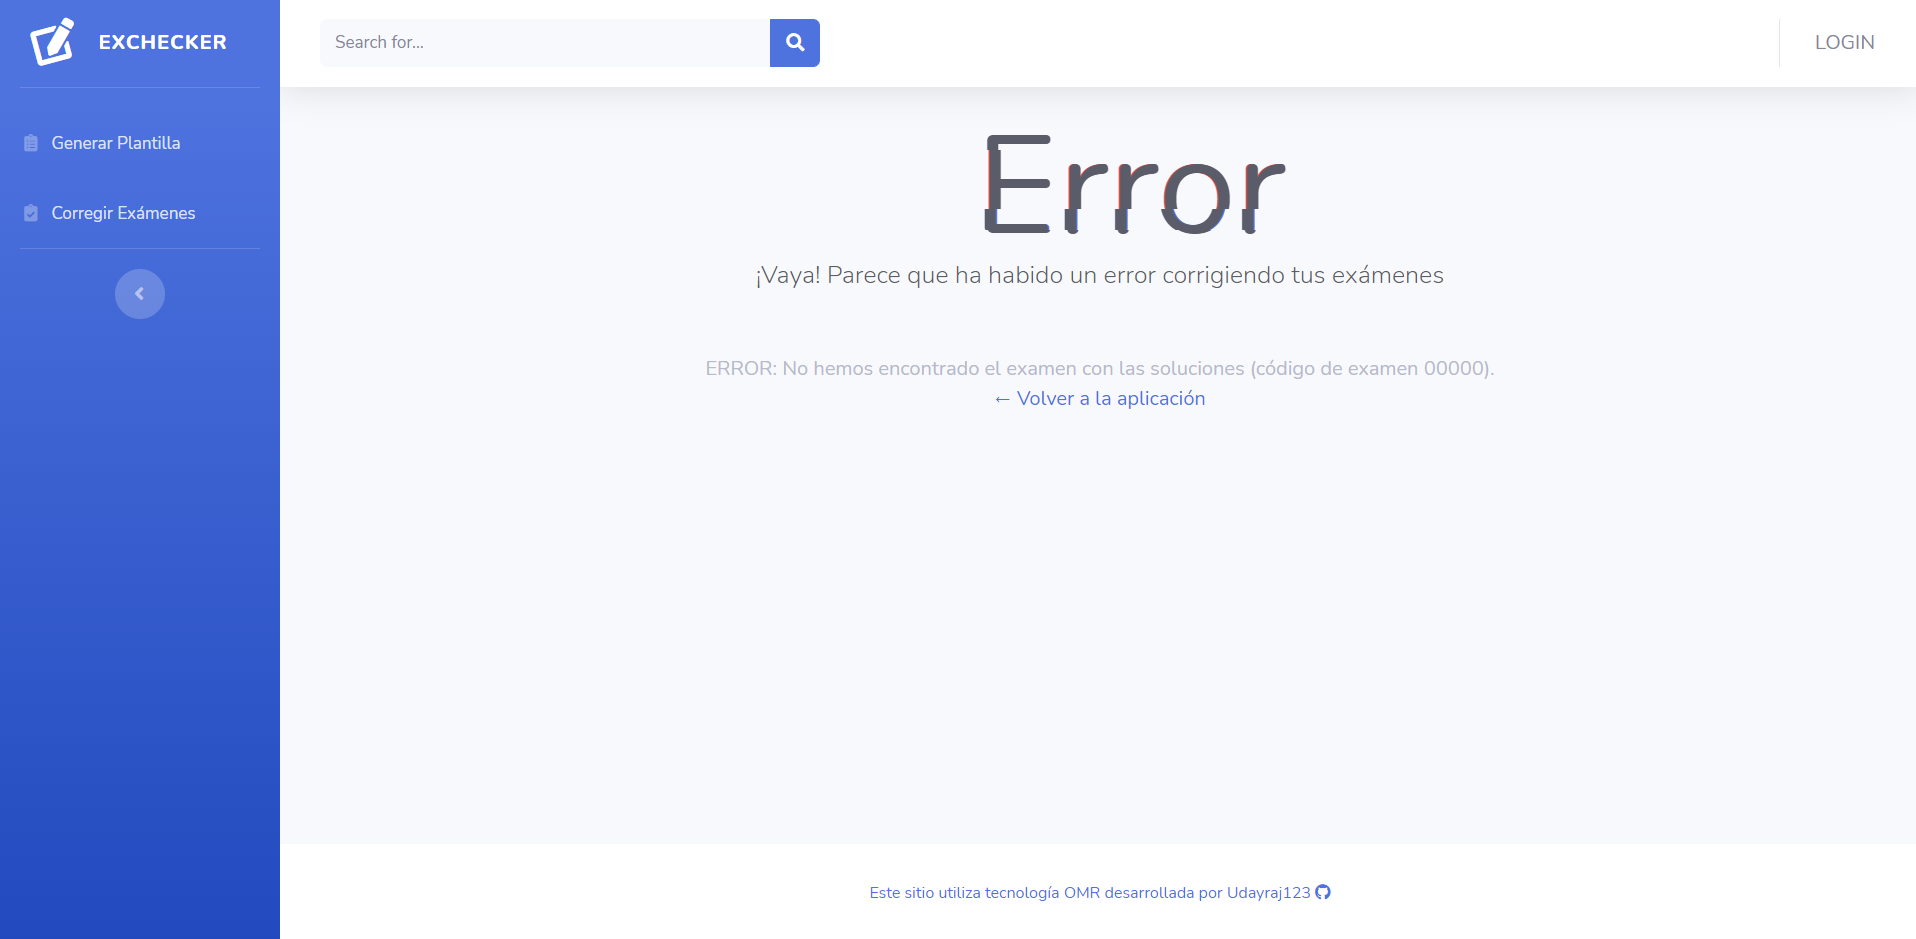
\includegraphics[width=12cm, keepaspectratio]{img/error_en_correccion}
  \caption{Página de error en corrección de exámenes}
  \label{figura:error_en_correccion}
\end{figure}

\section{Sistema de \textit{logging} y configuración} 
\label{sec:sistema_logging}

Uno de los objetivos iniciales al iniciar este proyecto fue la sostenibilidad y 
escalabilidad del mismo. Para asegurar esto, el proyecto cuenta con un fichero
de configuración
inicial que se lee al iniciar la aplicación. Este fichero de configuración permite
a la aplicación adaptarse a diferentes escenarios. El fichero de configuración
actual en ExChecker es el siguiente:

{\footnotesize
\begin{verbatim}
  {
    "checked_folder_tmp": "/tmp/exchecker/",
    "inputs_folder": "OMRChecker/inputs/",
    "omr_template": "./OMRChecker/template.json",
    "omr_main": "./OMRChecker/main.py",
    "output_dir": "./OMRChecker/outputs/",
    "csvs_dir": "./exchecker_app/static/csvs/",
    "templates_dir": "./exchecker_app/static/templates/",
    "loglevel": "DEBUG",
    "log_path": "./logs/log.txt",
    "users_log_path": "./logs/users_log.txt",
    "maxBytes_log": 50000,
    "backupCount": 3,
    "web_url": "127.0.0.1:8000",
    "marker_url": "http:127.0.0.1:8000/static/template_marker.jpg",
    "version_file": "./VERSION.txt"
  }
\end{verbatim}
}

\begin{comment}
\begin{figure}
  \centering
  \theverbbox
  \caption{Fichero de configuración utilizado por ExChecker}
  \label{verbbox:config_file}
\end{figure}
\end{comment}

Adicionalmente, desarrollamos un módulo generador de logs, que permitiese registrar
cualquier evento que se diese en la aplicación: generación de plantillas, correcciones
de exámenes, errores en ejecución\dots De esta forma la depuración del proyecto
es mucho más sencilla. Para la implementación del sistema de logs se ha utilizado
la librería de \textit{python} \textit{logging}\cite{logging:documentation}.
Un ejemplo de logs del sistema es el que puede observarse a continuación:

{\footnotesize
\begin{verbatim}
----------- INITIALIZING LOG EXCHECKER WEB APP -----------
Initializing log at 2021-06-22T19:27:14
The used log level is: DEBUG
The version is: 1.0

2021-06-22T19:27:14+0200 - INFO - Reading config file
2021-06-22T19:27:14+0200 - INFO - Config file read succsessfully
The used config is:
{
    "checked_folder_tmp": "/tmp/exchecker/",
    "inputs_folder": "OMRChecker/inputs/",
    "omr_template": "./OMRChecker/template.json",
    "omr_main": "./OMRChecker/main.py",
    "output_dir": "./OMRChecker/outputs/",
    "csvs_dir": "./exchecker_app/static/csvs/",
    "templates_dir": "./exchecker_app/static/templates/",
    "loglevel": "DEBUG",
    "log_path": "./logs/log.txt",
    "users_log_path": "./logs/users_log.txt",
    "maxBytes_log": 50000,
    "backupCount": 3,
    "web_url": "127.0.0.1:8000",
    "marker_url": "http:127.0.0.1:8000/static/template_marker.jpg",
    "version_file": "./VERSION.txt"
}
22-06-2021 19:27:20 - INFO - "GET / HTTP/1.1" 200 10717
22-06-2021 19:27:20 - INFO - "GET /css.css HTTP/1.1" 200 638
22-06-2021 19:27:23 - INFO - "GET /accounts/login/ HTTP/1.1" 200 5668
22-06-2021 19:27:23 - INFO - "GET /css.css HTTP/1.1" 200 638
22-06-2021 19:27:26 - INFO - "GET /get_template HTTP/1.1" 200 9796
22-06-2021 19:27:26 - INFO - "GET /css.css HTTP/1.1" 200 638
22-06-2021 19:27:26 - INFO - "GET /get_template.js HTTP/1.1" 200 1554
22-06-2021 19:27:29 - INFO - "GET /check_exams HTTP/1.1" 200 10745
22-06-2021 19:27:29 - INFO - "GET /css.css HTTP/1.1" 200 638
22-06-2021 19:27:29 - INFO - "GET /check_exams.js HTTP/1.1" 200 2436
22-06-2021 19:27:40 - INFO - "POST /upload_exams/ HTTP/1.1" 200 5
22-06-2021 19:27:51 - INFO - "POST /check_exams HTTP/1.1" 200 7550
22-06-2021 19:27:51 - INFO - "GET /css.css HTTP/1.1" 200 638
22-06-2021 19:27:54 - INFO - "GET / HTTP/1.1" 200 10717
22-06-2021 19:27:54 - INFO - "GET /css.css HTTP/1.1" 200 638
\end{verbatim}
}

\section{Despliegue de la aplicación} 
\label{sec:despliegue}

La aplicación ExChecker ha sido desarrollado con el objetivo de utilizarse en
un entorno local, es decir, cada usuario instala la aplicación en su ordenador y
posteriormente puede utilizarla.

Para el despliegue de la aplicación se ha utilizado la herramienta \textit{Docker}
\cite{docker:documentation} descrita
en la Sección~\ref{sec:docker}. Esta herramienta nos ha permitido simular un entorno
completo, llamado contenedor, en el que se ejecutará la aplicación web. Para la creación
del contenedor \textit{Docker} en primera instancia se debe instalar \textit{Docker} en el sistema
y crear un fichero \textit{Dockerfile}.
Este fichero contendrá instrucciones para la creación de la imagen de nuestro proyecto,
como módulos necesarios en la instalación, código fuente, dependencias, etc.
El fichero Dockerfile desarrollado para nuestro proyecto es el siguiente:

{\footnotesize
\begin{verbatim}
  FROM \textit{python}:3.7

  RUN apt-get update \
      && apt-get install -y --no-install-recommends \
          postgresql-client ffmpeg libsm6 libxext6 \
          \textit{python}3-opencv wkhtmltopdf \
          poppler-utils zip \
      && rm -rf /var/lib/apt/lists/*
  
  WORKDIR /app
  COPY . .
  RUN pip install -r requirements.txt
  EXPOSE 8000
  CMD ["python", "manage.py", "runserver", "0.0.0.0:8000", "--insecure"]
\end{verbatim}
}

Posteriormente ejecutamos el comando \textit{docker build} para construir la imagen
en base a las directrices del fichero \textit{Dockerfile}. Una vez construida la imagen,
iniciamos sesión en el sistema Docker con el comando \textit{docker login} y finalmente
procedemos a la subida de nuestra imagen: \textit{docker push adrianrio/exchecker}

En el Anexo~\ref{app:guia_instalacion} se explican los detalles para una instalación
correcta de la aplicación desde un sistema Windows.


%%%%%%%%%%%%%%%%%%%%%%%%%%%%%%%%%%%%%%%%%%%%%%%%%%%%%%%%%%%%%%%%%%%%%%%%%%%%%%%%
%%%%%%%%%%%%%%%%%%%%%%%%%%%%%%%%%%%%%%%%%%%%%%%%%%%%%%%%%%%%%%%%%%%%%%%%%%%%%%%%
% EXPERIMENTOS Y VALIDACIÓN %
%%%%%%%%%%%%%%%%%%%%%%%%%%%%%%%%%%%%%%%%%%%%%%%%%%%%%%%%%%%%%%%%%%%%%%%%%%%%%%%%

\cleardoublepage
\chapter{Experimentos y validación}

En este capítulo vamos a plasmar los experimentos y pruebas que has sido
realizados para poner a prueba la aplicación ExChecker, sobre todo
centrándonos en el sistema OMR.

\section{Subida de documentos escaneados}
\label{sec:doc_escaneados}

La manera de subir documentos adecuada a la plataforma es la subida de
documentos escaneados. Esto es así debido a que el sistema OMR no
tiene que delimitar el documento, únicamente tiene que encontrar las
marcas en los vértices y alinear el documento correctamente.

Como experimento se han utilizado documentos escaneados y se ha comprobado
que el sistema OMR es capaz de detectar las casillas de una forma
correcta. En la Figura~\ref{figura:test1} se puede observar un ejemplo
de documento escaneado subido y su posterior reconocimiento por parte
del sistema OMR.

\begin{figure}
  \centering
  \subfloat[Documento subido]{
  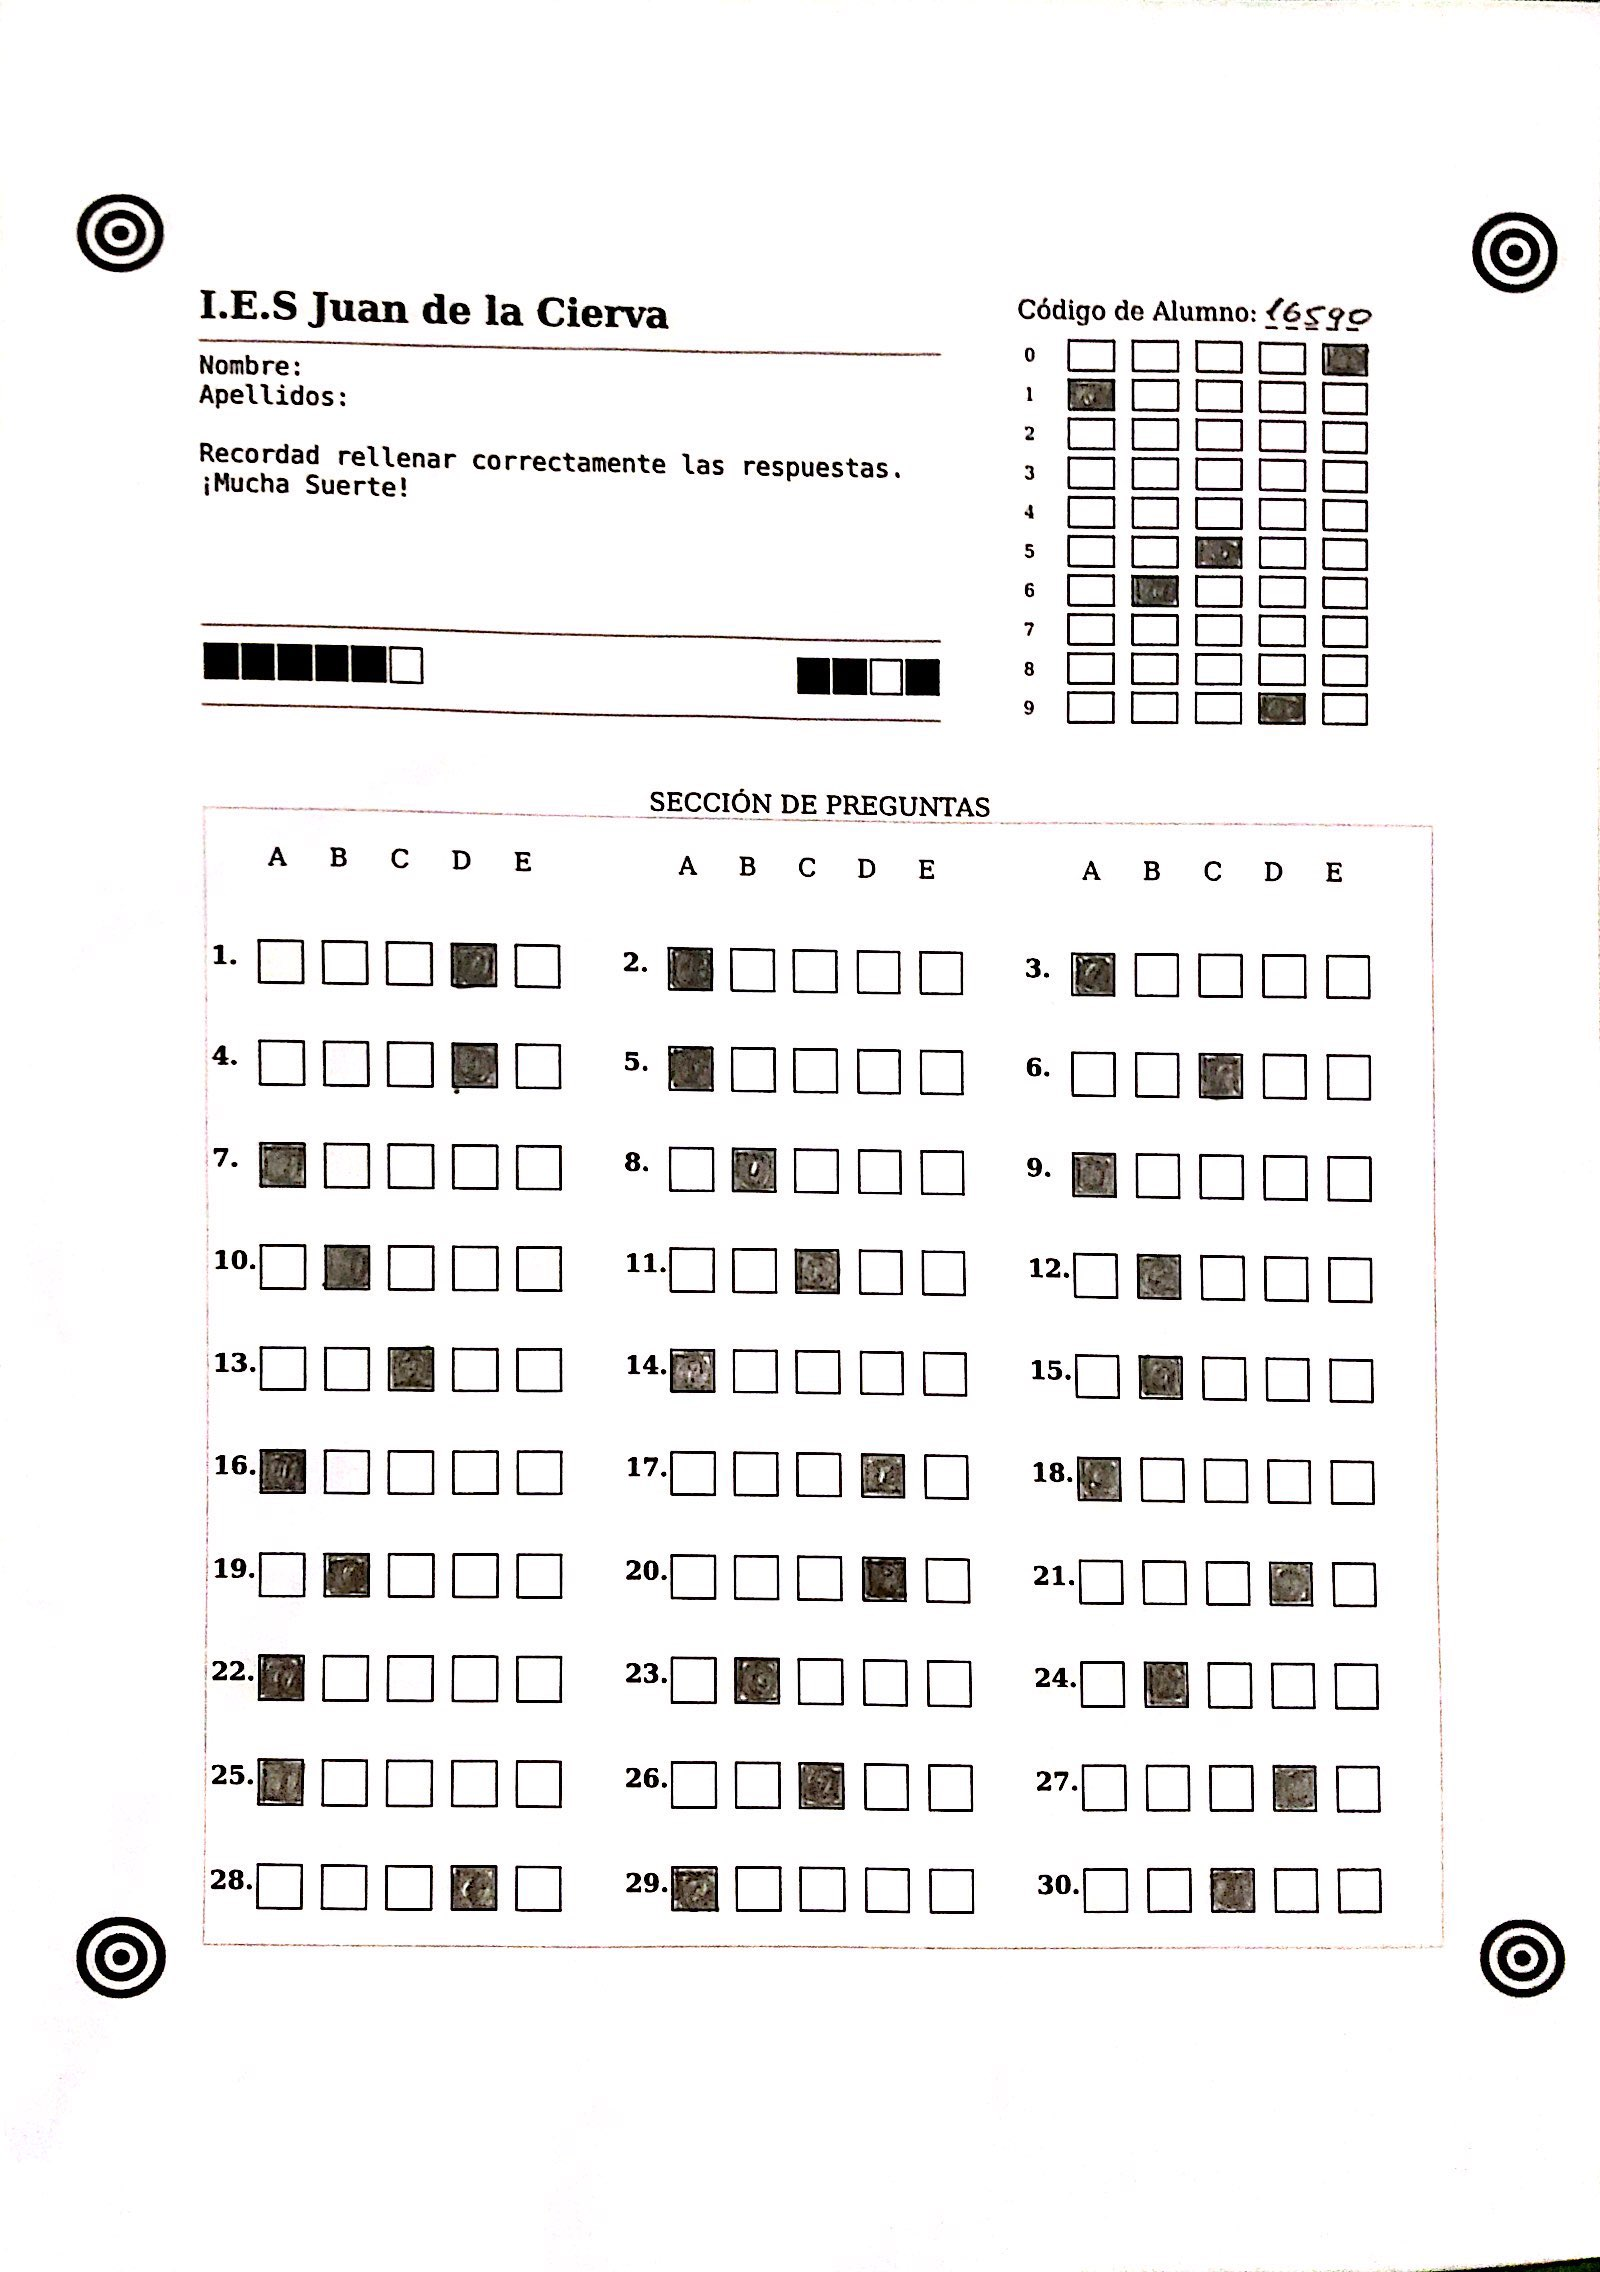
\includegraphics[width=8cm, height=11cm]{img/tests/test1_a} }
  \subfloat[Detección correcta]{
  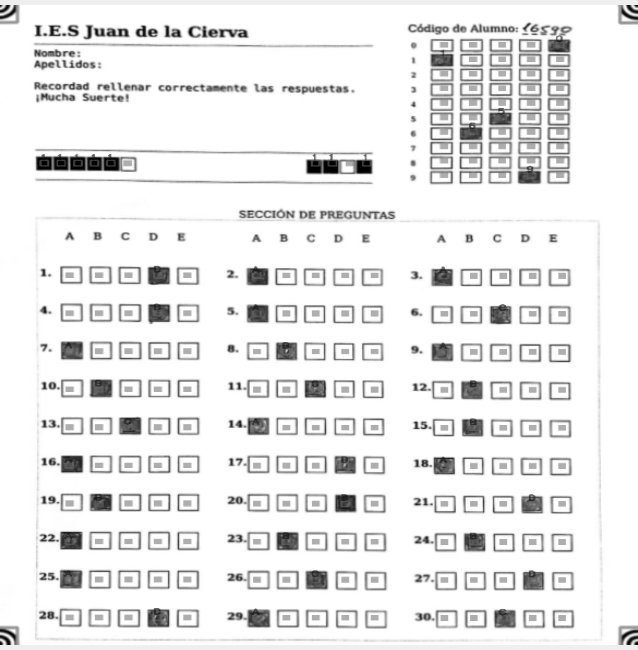
\includegraphics[width=8cm, height=11cm]{img/tests/test1_b} }
  \caption{Ejemplo de prueba realizada con documento escaneado}
  \label{figura:test1}
\end{figure}

\section{Subida de documentos fotografiados}
\label{sec:doc_fotografiados}

En este caso se va a comprobar el comportamiento del sistema OMR ante
documentos fotografiados. El sistema OMR debe ser capaz de delimitar los
documentos y orientarlos de una forma correcta.

\subsection{Fotografías bien alineadas}
\label{subsec:fotografias_vertical}

En general, el sistema OMR se comporta de manera correcta cuando los
documentos subidos están fotografiados correctamente alineados y a una
distancia adecuada. En la Figura~\ref{figura:test2} se puede observar un ejemplo
de documento fotografiado correctamente alineado y su posterior reconocimiento por parte
del sistema OMR.

\begin{figure}
  \centering
  \subfloat[Documento subido]{
  \includegraphics[width=8cm, height=11cm]{img/tests/test2_a} }
  \subfloat[Detección correcta]{
  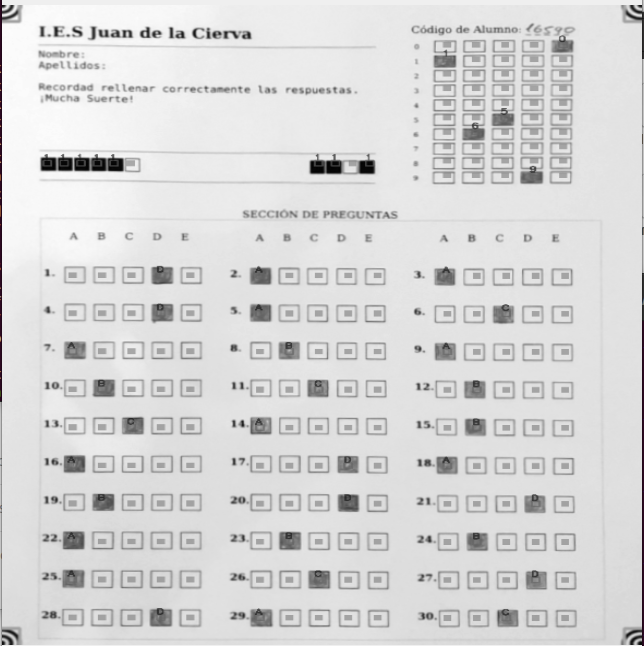
\includegraphics[width=8cm, height=11cm]{img/tests/test2_b} }
  \caption{Ejemplo de prueba realizada con documento fotografiado correctamente alineado}
  \label{figura:test2}
\end{figure}

\subsection{Fotografías en oblicuo}
\label{subsec:fotografias_oblicuo}

En este caso el sistema OMR tiene dificultades para alinear los documentos
y puede ser que las posiciones de las casillas de respuestas no encajen
con su plantilla. Dependiendo del grado de inclinación de la fotografía
el sistema será capaz de ubicar correctamente las casillas o no.
En la Figura~\ref{figura:test3} se puede observar un ejemplo
de documento fotografiado de manera oblicua y su posterior
reconocimiento por parte
del sistema OMR. En este caso, el reconocimiento de la sección de
codificación de información no es el correcto, por lo tanto la
plataforma descartaría el documento.

\begin{figure}
  \centering
  \subfloat[Documento subido]{
  \includegraphics[width=8cm, height=11cm]{img/tests/test3_a} }
  \subfloat[Detección de un error]{
  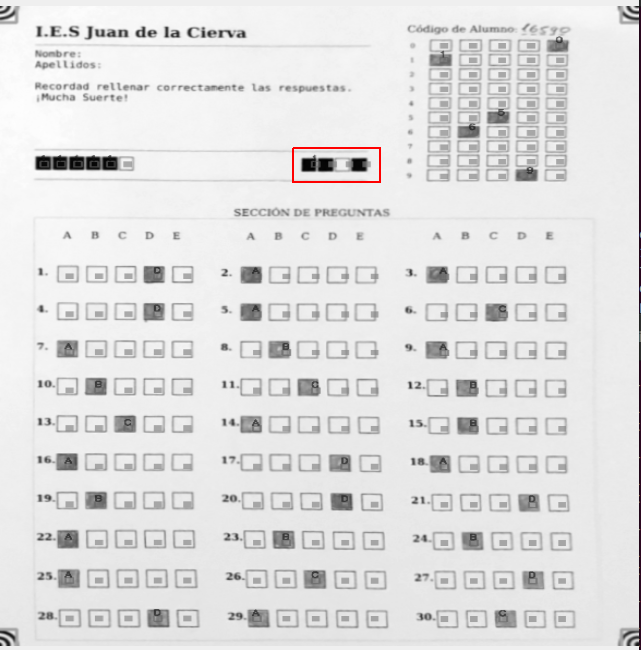
\includegraphics[width=8cm, height=11cm, ]{img/tests/test3_b} }
  \caption{Ejemplo de prueba realizada con documento fotografiado de manera oblicua}
  \label{figura:test3}
\end{figure}

\subsection{Fotografías alineadas con rotación}
\label{subsec:fotografias_rotación}

En el caso de documentos fotografiados con una alineación correcta y cierto
grado de rotación el sistema OMR no es capaz de encontrar los límites del
documento. En la Figura~\ref{figura:test7} se puede observar un ejemplo
de documento fotografiado con alineación correcta y un
grado de rotación de 30º y su posterior
reconocimiento por parte
del sistema OMR.

\begin{figure}
  \centering
  \subfloat[Documento subido]{
  \includegraphics[width=8cm, height=11cm]{img/tests/test7_a} }
  \subfloat[No se delimita el documento]{
  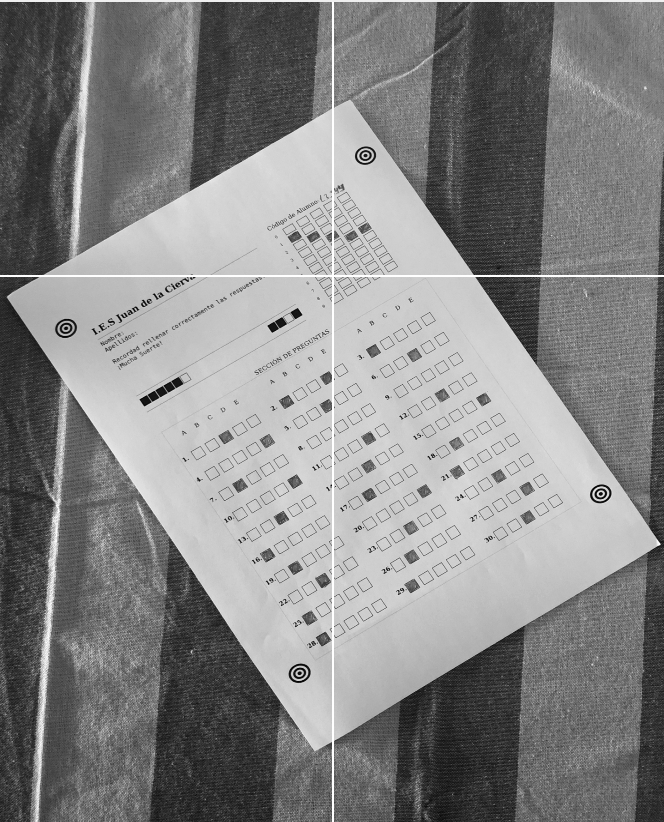
\includegraphics[width=8cm, height=11cm, ]{img/tests/test7_b} }
  \caption{Ejemplo de prueba fallida. El sistema no es capaz de delimitar el documento}
  \label{figura:test7}
\end{figure}

\subsection{Fotografías con sombras}
\label{subsec:fotografias_sombras}

En el caso en el que existan sombras en los documentos escaneados, el
sistema OMR puede que detecte alguna sombra como marcas de tinta en el
documento. Además, en el caso de que la sombra no sea uniforme en todo el
documento puede influir en otras respuestas del mismo.
En la Figura~\ref{figura:test4} se puede observar un ejemplo
de documento fotografiado con sombras y su posterior
reconocimiento por parte
del sistema OMR.
En este caso, se puede apreciar como el sistema reconoce como marcas
las respuestas D de la primera columna de preguntas.

\begin{figure}
  \centering
  \subfloat[Documento subido]{
  \includegraphics[width=8cm, height=11cm]{img/tests/test4_a} }
  \subfloat[Detección de un error]{
  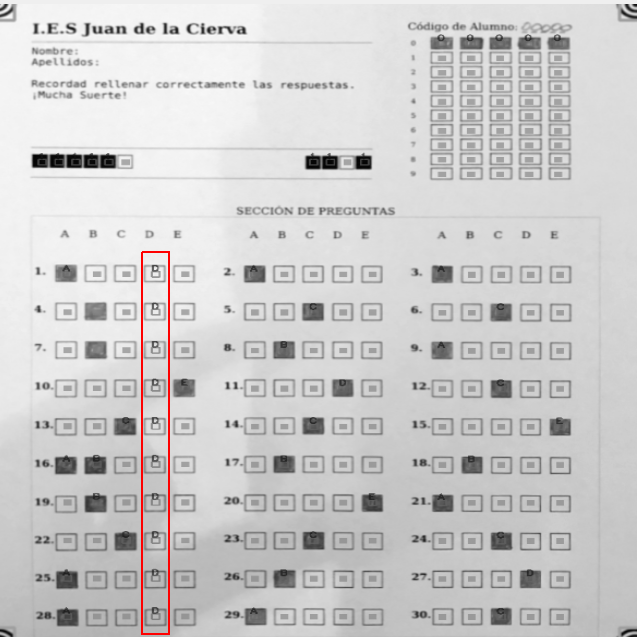
\includegraphics[width=8cm, height=11cm]{img/tests/test4_b} }
  \caption{Ejemplo de prueba fallida. Las sompras se interpretan como respuestas}
  \label{figura:test4}
\end{figure}

\section{Documentos a bolígrafo y uso del Tipp-Ex}
\label{sec:boli_tipex}

El sistema OMR se comporta correctamente en el caso de que los exámenes estén
rellenados con bolígrafo en vez de con lapicero. En el caso del uso del
Tipp-Ex el sistema detecta las respuestas como respuestas vacías, por lo
que el comportamiento es el correcto.
En la Figura~\ref{figura:test5} se
puede observar un ejemplo
de documento rellenado con bolígrafo y el uso del Tipp-Ex en él.

\begin{figure}
  \centering
  \subfloat[Documento subido]{
  \includegraphics[width=8cm, height=11cm]{img/tests/test5_a} }
  \subfloat[Detección correcta]{
  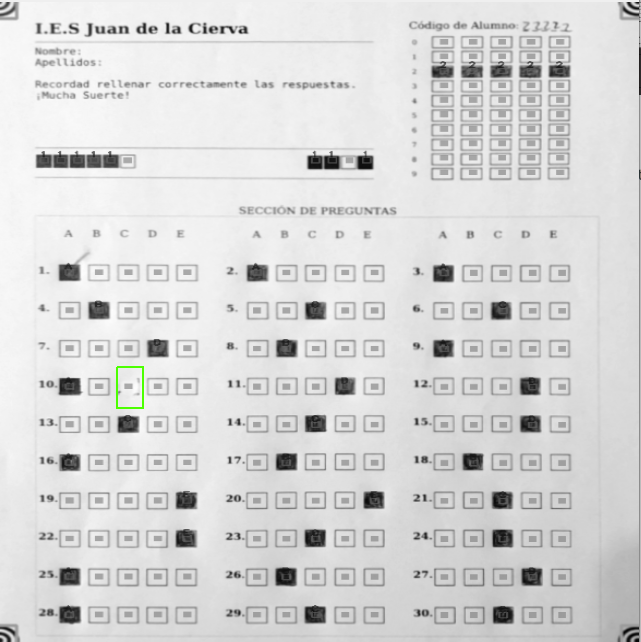
\includegraphics[width=8cm, height=11cm]{img/tests/test5_b} }
  \caption{Ejemplo de prueba realizada con documento rellenado a bolígrafo y Tipp-Ex}
  \label{figura:test5}
\end{figure}

\section{Casillas no rellenadas completamente}
\label{sec:casillas_con_cruz}

En el caso de que las casillas de respuestas no estén rellenadas de forma
completa, es decir, se utilice por ejemplo una equis para su marcado, el
sistema OMR puede detectarlas. Aún así, esta no es la forma recomendada
de rellenar las plantillas que ExChecker genera.
En la Figura~\ref{figura:test6} se puede observar un ejemplo
de documento fotografiado con casillas no rellenadas completamente
reconocimiento por parte
del sistema OMR.

\begin{figure}
  \centering
  \subfloat[Documento subido]{
  \includegraphics[width=8cm, height=11cm]{img/tests/test6_a} }
  \subfloat[Detección correcta]{
  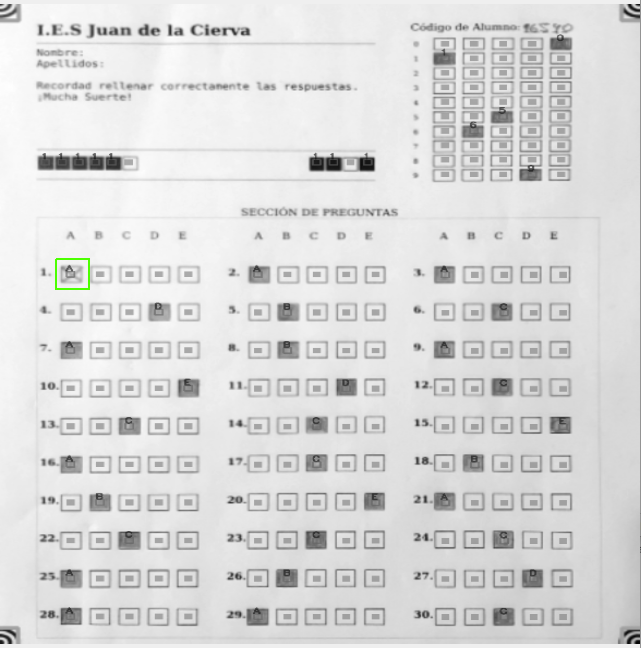
\includegraphics[width=8cm, height=11cm]{img/tests/test6_b} }
  \caption{Ejemplo de prueba realizada con documento con casillas no rellenadas completamente}
  \label{figura:test6}
\end{figure}

\section{Resultados}
\label{sec:resultados}

Como conclusiones de los experimentos y pruebas realizadas obtenemos las
siguiente conclusiones:

\begin{enumerate}
  \item Se prefiere la subida de documentos escaneados a documentos fotografiados,
  ya que el sistema en el caso de los primeros es más robusto frente a errores. 
  \item Los documentos fotografiados bien alineados son detectados correctamente
  por el sistema OMR.
  \item Los documentos fotografiados de manera oblicua dependen del grado de inclinación
  para que sean correctamente detectados por el sistema.
  \item En el caso de documentos fotografiados con sombras es posible que el sistema no
  consiga detectar las respuestas correctamente.
  \item En cuanto a las pruebas realizadas comprobando el uso de bolígrafo y Tipp-Ex en
  los documentos, éstas nos indican que el sistema reconoce estos documentos perfectamente.
  \item Finalmente, las casillas de respuestas que no están rellenada de forma completa
  no se recomiendan, aunque el sistema OMR es capaz de detectarlas.
\end{enumerate}

%%%%%%%%%%%%%%%%%%%%%%%%%%%%%%%%%%%%%%%%%%%%%%%%%%%%%%%%%%%%%%%%%%%%%%%%%%%%%%%%
%%%%%%%%%%%%%%%%%%%%%%%%%%%%%%%%%%%%%%%%%%%%%%%%%%%%%%%%%%%%%%%%%%%%%%%%%%%%%%%%
% CONCLUSIONES %
%%%%%%%%%%%%%%%%%%%%%%%%%%%%%%%%%%%%%%%%%%%%%%%%%%%%%%%%%%%%%%%%%%%%%%%%%%%%%%%%

\cleardoublepage
\chapter{Conclusiones}
\label{chap:conclusiones}

En este capítulo se indican las conclusiones extraídas en el desarrollo
de la aplicación, así como la valoración de los objetivos cumplidos.
Además, se incluirán los conocimientos aplicados y aprendidos en todo
el desarrollo del proyecto.
Finalmente comentaremos los trabajos futuros de este proyecto.

\section{Consecución de objetivos}
\label{sec:consecucion-objetivos}

Al inicio de esta memoria se comentaba en el
Capítulo~\ref{chap:objetivos} los objetivos
propuestos para ser alcanzados.

El objetivo general del proyecto
consistía en la elaboración de una aplicación web que, haciendo uso
de la tecnología OMR, fuese capaz de corregir exámenes tipo test
de una manera totalmente automática. Este objetivo ha sido cumplido
tal y como puede observarse a lo largo de esta memoria.

Para la cumplimentación del objetivo general se partía de varios
objetivos específicos: flexibilidad en la generación de plantillas,
aplicación web responsiva, sistema de usuarios, y finalmente la
aplicación debía ser lo más intuitiva y fácil de manejar posible.

Todos estos objetivos han sido cumplidos haciendo uso de varias
herramientas que se muestran en el proyecto, creando así un sistema
totalmente modular que incluye varias herramientas que nos han
permitido la cumplimentación de todos estos objetivos.

\begin{comment}
Y si has llegado hasta aquí, siempre es bueno pasarle el corrector ortográfico, que las erratas quedan fatal en la memoria final.
Para eso, en Linux tenemos aspell, que se ejecuta de la siguiente manera desde la línea de \emph{shell}:

\begin{verbatim}
  aspell --lang=es_ES -c memoria.tex
\end{verbatim}
\end{comment}

\section{Aplicación de lo aprendido}
\label{sec:aplicacion}

En esta sección comentaremos los conocimientos que se han aplicado
para el desarrollo del proyecto.

Como puede observarse, el proyecto requiere una gran cantidad de
conocimientos en tecnologías web. Se ha necesitado comprender
profundamente los protocolos de comunicación en estos entornos (HTTP),
y sobre todo las herramientas que hacen necesaria la visualización
de contenidos web en navegadores de usuarios: HTML, CSS, JavaScript.

Además, ha sido importante un conocimiento en el desarrollo en \textit{python}
y la utilización de un \textit{framework} web como \textit{Django}.

\section{Lecciones aprendidas}
\label{sec:lecciones_aprendidas}

En este proyecto hemos aprendido muchas herramientas y tecnologías
útiles que, una vez integradas en un sistema global, nos han permitido
alcanzar los objetivos propuestos. Estas son algunas de las lecciones
aprendidas:

\begin{enumerate}
  \item Librería \textit{logging} en \textit{python}: Esta librería ha sido un descubrimiento
  muy útil, ya que nos ha permitido un desarrollo mucho más limpio y sobretodo
  una depuración del código mucho más rápida.
  \item Sistema OMR: Hemos aprendido en este proyecto como funciona un
  sistema basado en OMR y qué utilidades tiene.
  \item Conversión de documentos HTML a PDF: Utilizando la herramienta
  Wkhtmltopdf y el módulo de \textit{python} \textit{Pdfkit} hemos conseguido convertir
  documentos HTML en documentos en PDF. Esta es una de las muchas
  herramientas que no se conocían al iniciar este proyecto. 
  \item Subida de documentos en web: Gracias a la herramienta \textit{Filepond}
  nos hemos adentrado en el funcionamiento de subida de documentos
  en la web.
  \item Despliegue de aplicación: Como comentábamos anteriormente,
  el despliegue de la aplicación se ha realizado gracias a Docker,
  un sistema de virtualización que te permite ejecutar programas
  en un entorno completamente virtualizado.
\end{enumerate}


\section{Trabajos futuros}
\label{sec:trabajos_futuros}

A continuación se muestran
algunas tareas y trabajos futuros
a retomar:

\begin{enumerate}
  \item Despliegue global de la aplicación: Por el momento la aplicación
  ExChecker únicamente está disponible para ser ejecutada en entornos locales.
  Una nueva forma de despliegue es posible, como por ejemplo utilizar
  un servidor web público para que la aplicación esté accesible a cualquier
  usuario con tal de que disponga de un navegador web.
  \item Utilización de correo para registro y recuperación de contraseñas:
  Sería posible que cada vez que un nuevo usuario se registrase en la aplicación
  se le enviase un correo electrónico de confirmación. De esta forma se evitaría
  la generación de cuentas obsoletas. Adicionalmente, en el ámbito de
  restauración de contraseñas, sería posible enviar un correo electrónico
  de restauración de contraseña al usuario que lo solicite. De esta forma
  el sistema sería mucho menos vulnerable y más robusto.
  \item Optimización en errores en corrección de exámenes: Algo posible
  sería que no se abortase la corrección de exámenes en algunas situaciones.
  Si un examen no se ha podido corregir correctamente se le puede indicar
  al usuario a que fichero corresponde y proseguir con la corrección. Adicionalmente
  se puede redactar un informe con información relevante a la corrección
  de los exámenes, que incluya la hora de inicio, la hora de finalización,
  posibles errores encontrados, etc. Además, se podría incluir una imagen del examen
  que ha sido rechazado.
  \item Revisión en los mensajes de logs: Los mensajes de logs son los que
  nos indican el flujo de nuestro programa y las posibles vulnerabilidades
  que éste tiene. Tener un sistema de logs que informe de una manera clara
  y concisa el flujo de ejecución y los errores que se manifiesten en el código
  decrementa
  el tiempo invertido en busca de errores.
  \item Gestión automática de permutaciones de un mismo examen: Incluyendo
  esta caractarística, se aseguraría la integridad académica de las
  pruebas y se evitarían posibles plagios.

\end{enumerate}


%%%%%%%%%%%%%%%%%%%%%%%%%%%%%%%%%%%%%%%%%%%%%%%%%%%%%%%%%%%%%%%%%%%%%%%%%%%%%%%%
%%%%%%%%%%%%%%%%%%%%%%%%%%%%%%%%%%%%%%%%%%%%%%%%%%%%%%%%%%%%%%%%%%%%%%%%%%%%%%%%
% APÉNDICE(S) %
%%%%%%%%%%%%%%%%%%%%%%%%%%%%%%%%%%%%%%%%%%%%%%%%%%%%%%%%%%%%%%%%%%%%%%%%%%%%%%%%

\cleardoublepage
\appendix

\chapter{Guía De Instalación}
\label{app:guia_instalacion}

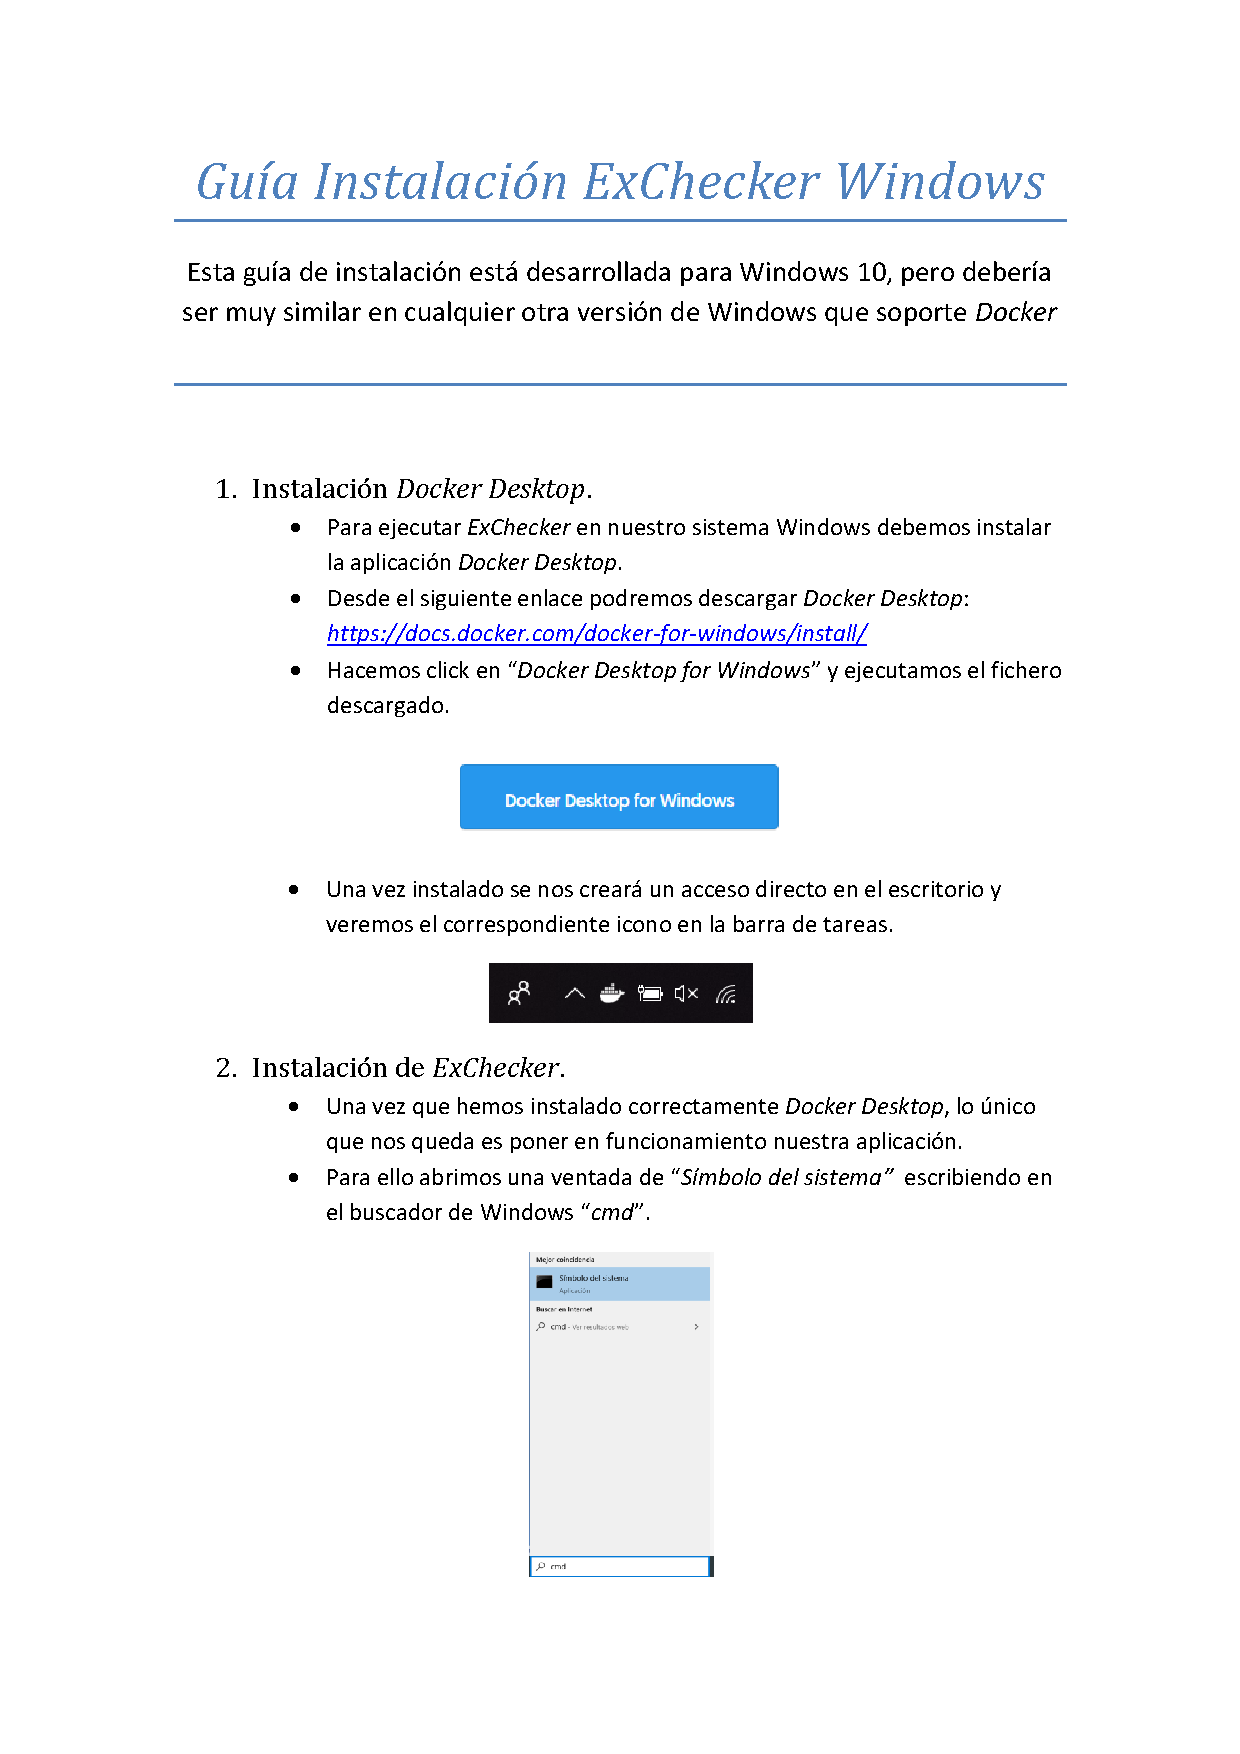
\includepdf[pages=-]{pdf/guia_instalacion}

\chapter{Guía Para Profesores}
\label{app:guia_profesores}

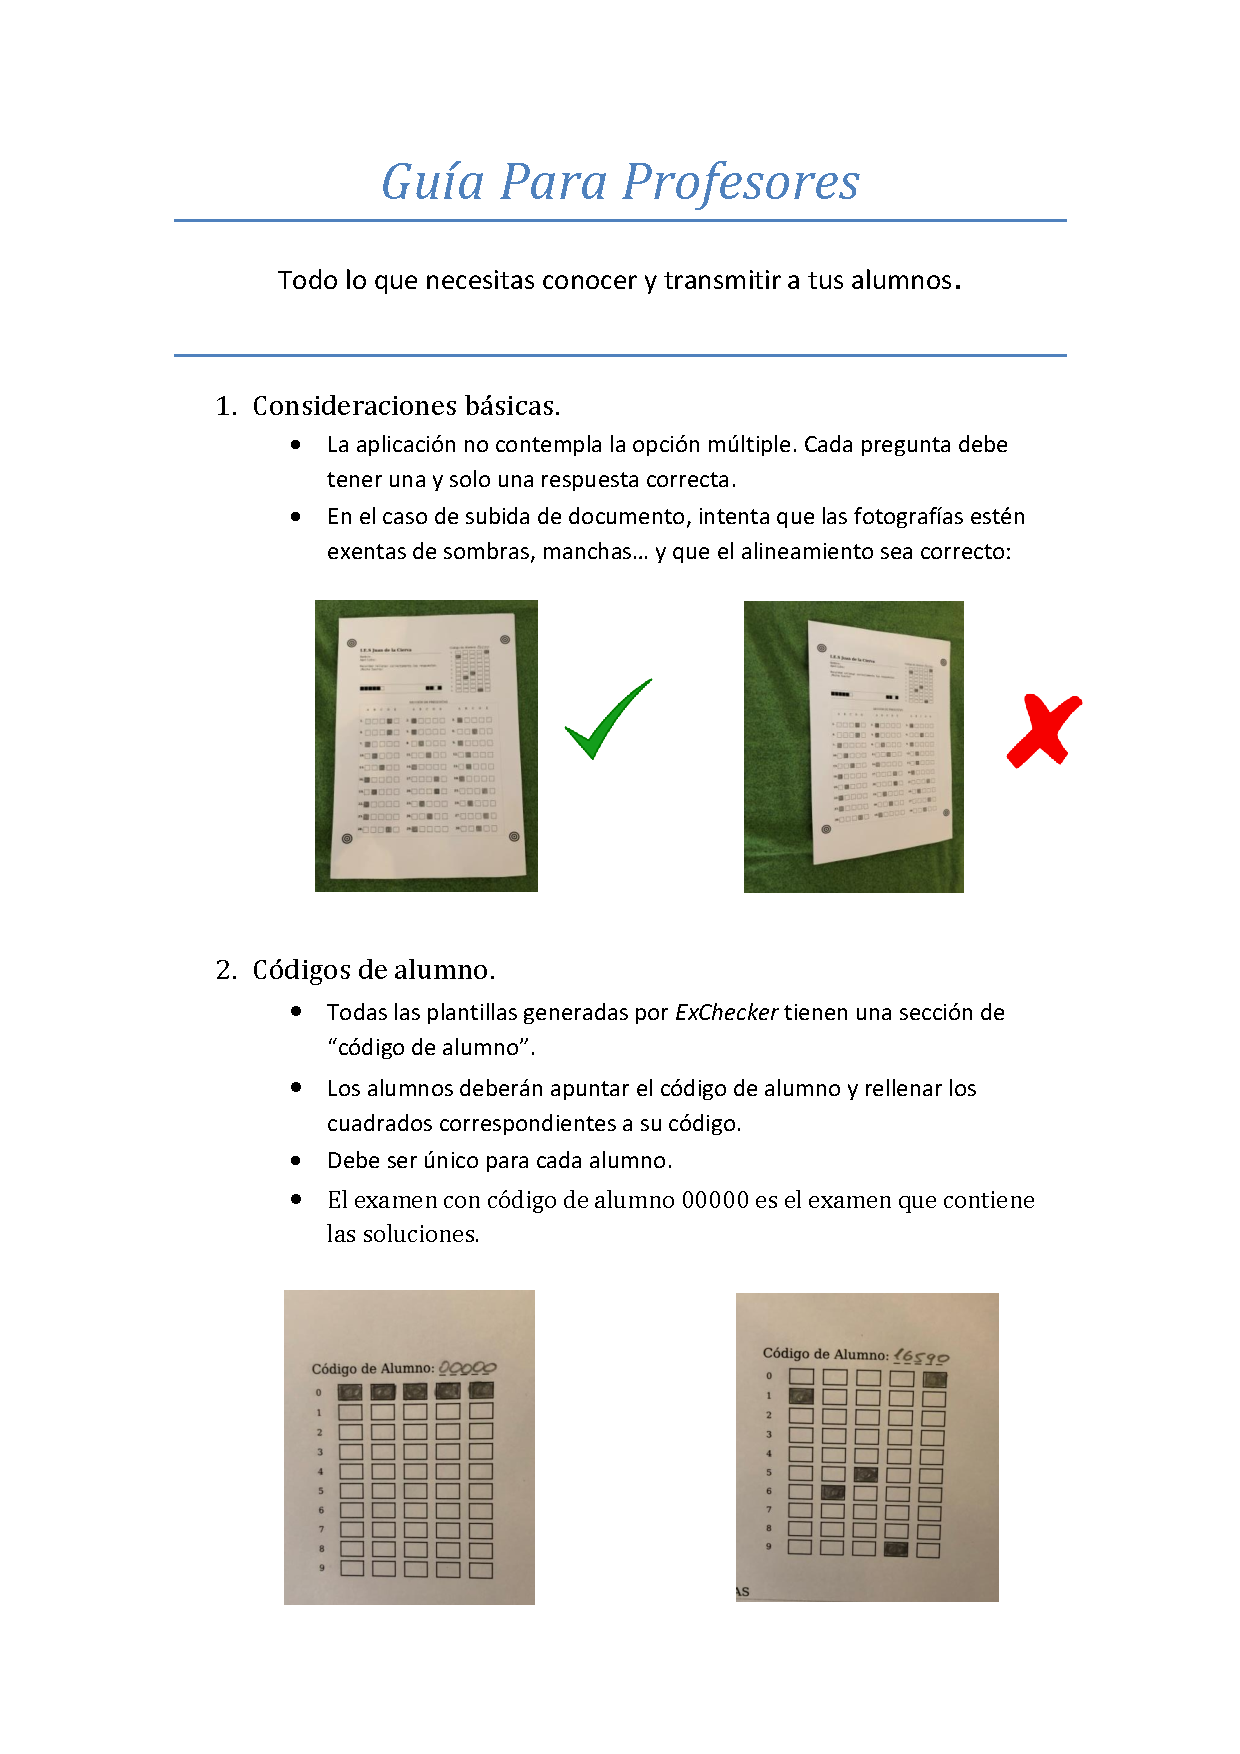
\includepdf[pages=-]{pdf/guia_para_profesores}

\chapter{Guía Para Alumnos}
\label{app:guia_alumnos}

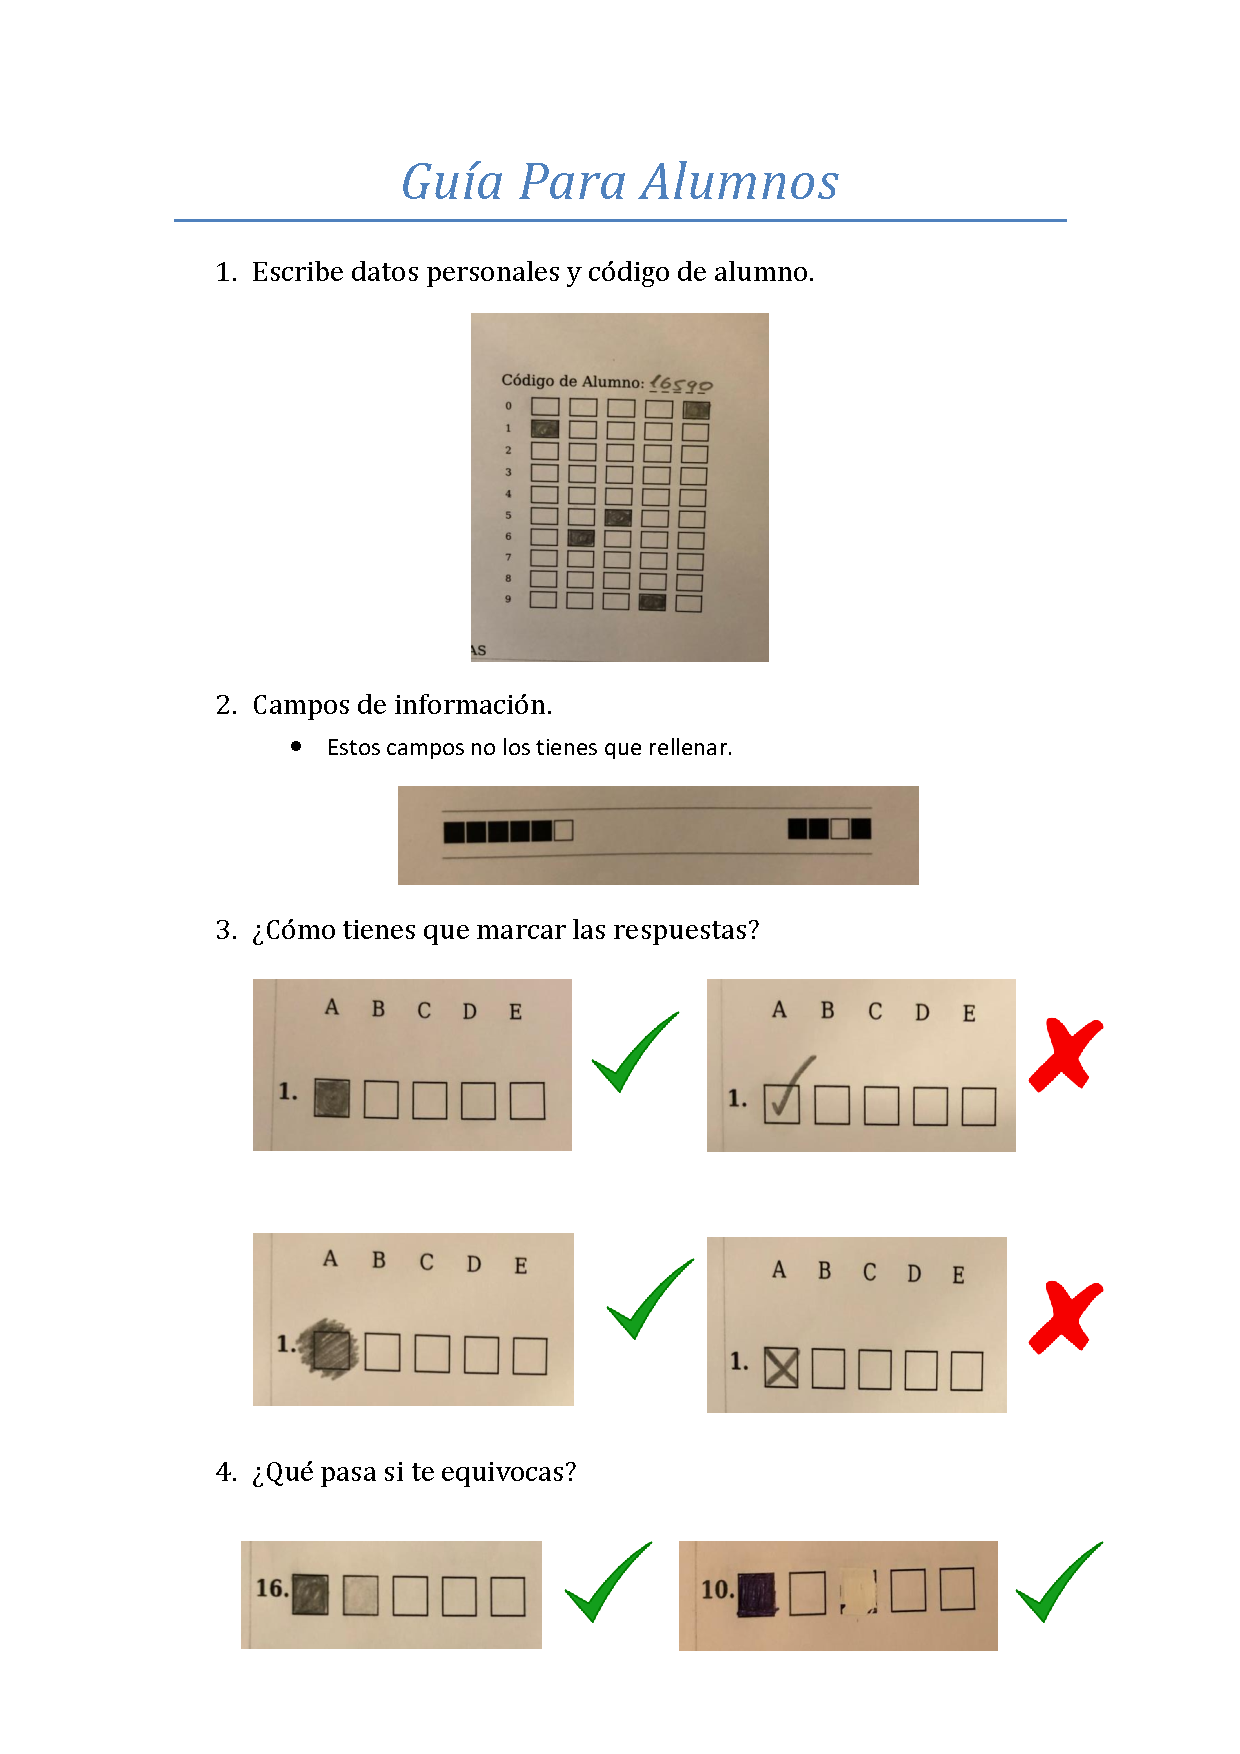
\includepdf[pages=-]{pdf/guia_para_alumnos}

\chapter{API de comunicaciones}
\label{app:api}

\begin{longtable}{ | p{5cm} | p{2cm} | p{7cm} |}
  %Cabecera
  \caption{API de comunicaciones}
  \label{tabla:api} \\ \hline
  \multicolumn{3}{|c|}{\textbf{API de comunicaciones}} \\
  \hline
  \centering \textbf{Recurso} & \centering \textbf{Operación} & \centering \textbf{Semántica} \tabularnewline
  \hline
  \endfirsthead

  \caption{API de comunicaciones (continuación)} \\ \hline
  \multicolumn{3}{|c|}{\textbf{API de comunicaciones (continuación)}} \\
  \hline
  \centering \textbf{Recurso} & \centering \textbf{Operación} & \centering \textbf{Semántica} \tabularnewline
  \hline
  \endhead
  \hline

  \multicolumn{3}{|r|}{\small \textit{Exchecker API}} \\
  \hline
  \endfoot
  \hline

  \multicolumn{3}{|r|}{\small \textit{ExChecker API}} \tabularnewline
  \hline
  \endlastfoot

  %Contenido
  \centering / & \centering GET & \centering Página principal de la aplicación \tabularnewline

  \hline
  \centering \multirow{2}{*} {/get\_template}
  & \centering GET & \centering Página generación de plantilla \tabularnewline
  \cline{2-3}
  & \centering POST & \centering Generación de plantilla \tabularnewline

  \hline
  \centering \multirow{2}{*} {/check\_exams}
  & \centering GET & \centering Página corrección de exámenes \tabularnewline
  \cline{2-3}
  & \centering POST & \centering Corrección de exámenes (visualiza estadísticas y resultados al finalizar) \tabularnewline

  \hline
  \centering \multirow{2}{*} {/my\_templates}
  & \centering GET & \centering Página de plantillas de usuario (necesidad de estar registrado y tener una sesión activa) \tabularnewline
  \cline{2-3}
  & \centering POST & \centering Eliminación de plantilla de usuario \tabularnewline

  \hline
  \centering /download\_all\_templates & \centering POST & \centering Descarga todas las plantillas para el usuario con la sesión activa en formato .zip \tabularnewline

  \hline
  \centering /upload\_exams & \centering POST & \centering Recurso utilizado por FilePond. Permite la subida de documentos \tabularnewline

  \hline
  \centering /get\_progress\_template & \centering POST & \centering Obtiene el progreso en la generación de plantillas \tabularnewline

  \hline
  \centering \multirow{2}{*} {/accounts/login/}
  & \centering GET & \centering Página de inicio de sesión \tabularnewline
  \cline{2-3}
  & \centering POST & \centering Inicio de sesión de usuario \tabularnewline

  \hline
  \centering /accounts/logout/ & \centering POST & \centering Cierre de sesión del usuario \tabularnewline

  \hline
  \centering \multirow{2}{*} {/accounts/register/}
  & \centering GET & \centering Página registro usuario \tabularnewline
  \cline{2-3}
  & \centering POST & \centering Registra al usuario en el sistema \tabularnewline

  \hline
  \centering \multirow{2}{*} {/accounts/forgot\_password/}
  & \centering GET & \centering Página de recuperación de contraseña \tabularnewline
  \cline{2-3}
  & \centering POST & \centering Permite la restauración de la contraseña en base al email proporcionado \tabularnewline

  \hline
  \centering /accounts/restore\_password/ & \centering POST & \centering Restaura la contraseña del usuario \tabularnewline
\end{longtable}

\chapter{Fichero de secciones de plantilla para OMR}
\label{app:template_json}

En este fichero JSON se definen las secciones en las que el sistema OMR
se fijará para obtener las respuestas.

A continuación se describen algunos valores de este fichero:

\begin{itemize}
  \item BubbleDimensions: Corresponde a las dimensiones de los rectángulos
  de las respuestas.
  \item Concatenations: Indicamos que los campos roll0, roll1, roll2\dots
  se concatenen en un único campo Roll al obtener los resultados en .csv.
  \item Singles: Definimos valores que no deben ser concatenados y deben
  considerarse individuales.
  \item QBlocks: Se especifican los bloques de respuestas para el sistema OMR.
  Entre ellos podemos destacar el bloque de código de alumno ``Roll'', o el
  bloque de codificación de información del examen ``questions\_info''.
\end{itemize}

{\footnotesize
\begin{verbatim}
  {
    "Dimensions": [
      1653,
      2339
    ],
    "BubbleDimensions": [
      25,
      25
    ],
    "Options": {
      "Marker": {
        "RelativePath": "omr_marker.jpg",
        "SheetToMarkerWidthRatio": 17
      }
    },
    "Concatenations": {
      "Roll": [
        "roll0",
        "roll1",
        "roll2",
        "roll3",
        "roll4"
      ]
    },
    "Singles": [
      "qi1",
      "qi2",
      "qi3",
      "qi4",
      "qi5",
      "qi6",
      "ri1",
      "ri2",
      "ri3",
      "ri4",
      "q1",
      "q2",
      "q3",
      "q4",
      "q5",
      "q6",
      "q7",
      "q8",
      "q9",
      "q10",
      "q11",
      "q12",
      "q13",
      "q14",
      "q15",
      "q16",
      "q17",
      "q18",
      "q19",
      "q20",
      "q21",
      "q22",
      "q23",
      "q24",
      "q25",
      "q26",
      "q27",
      "q28",
      "q29",
      "q30"
    ],
    "QBlocks": {
      "Roll": {
        "qType": "QTYPE_ROLL",
        "orig": [
          1137,
          133
        ],
        "bigGaps": [
          1,
          1
        ],
        "gaps": [
          75,
          53
        ],
        "qNos": [
          [
            [
              "roll0",
              "roll1",
              "roll2",
              "roll3",
              "roll4"
            ]
          ]
        ]
      },
      "questions_info": {
        "qType": "QTYPE_INT1",
        "orig": [
          105,
          566
        ],
        "bigGaps": [
          43.8,
          0
        ],
        "gaps": [
          36,
          36
        ],
        "qNos": [
          [
            [
              "qi1"
            ],
            [
              "qi2"
            ],
            [
              "qi3"
            ],
            [
              "qi4"
            ],
            [
              "qi5"
            ],
            [
              "qi6"
            ]
          ]
        ]
      },
      "responses_info": {
        "qType": "QTYPE_INT1",
        "orig": [
          805,
          566
        ],
        "bigGaps": [
          44,
          0
        ],
        "gaps": [
          36,
          36
        ],
        "qNos": [
          [
            [
              "ri1"
            ],
            [
              "ri2"
            ],
            [
              "ri3"
            ],
            [
              "ri4"
            ]
          ]
        ]
      },
      "MCQBlock1": {
        "qType": "QTYPE_MCQ5",
        "orig": [
          170,
          975
        ],
        "bigGaps": [
          180,
          -1250
        ],
        "gaps": [
          76,
          139
        ],
        "qNos": [
          [
            [
              "q1",
              "q4",
              "q7",
              "q10",
              "q13",
              "q16",
              "q19",
              "q22",
              "q25",
              "q28"
            ],
            [
              "q2",
              "q5",
              "q8",
              "q11",
              "q14",
              "q17",
              "q20",
              "q23",
              "q26",
              "q29"
            ],
            [
              "q3",
              "q6",
              "q9",
              "q12",
              "q15",
              "q18",
              "q21",
              "q24",
              "q27",
              "q30"
            ]
          ]
        ]
      }
    }
  }
\end{verbatim}
}

%%%%%%%%%%%%%%%%%%%%%%%%%%%%%%%%%%%%%%%%%%%%%%%%%%%%%%%%%%%%%%%%%%%%%%%%%%%%%%%%
%%%%%%%%%%%%%%%%%%%%%%%%%%%%%%%%%%%%%%%%%%%%%%%%%%%%%%%%%%%%%%%%%%%%%%%%%%%%%%%%
% BIBLIOGRAFIA %
%%%%%%%%%%%%%%%%%%%%%%%%%%%%%%%%%%%%%%%%%%%%%%%%%%%%%%%%%%%%%%%%%%%%%%%%%%%%%%%%

\cleardoublepage

% Las siguientes dos instrucciones es todo lo que necesitas
% para incluir las citas en la memoria
\bibliographystyle{abbrv}
\bibliography{memoria}  % memoria.bib es el nombre del fichero que contiene
% las referencias bibliográficas. Abre ese fichero y mira el formato que tiene,
% que se conoce como BibTeX. Hay muchos sitios que exportan referencias en
% formato BibTeX. Prueba a buscar en http://scholar.google.com por referencias
% y verás que lo puedes hacer de manera sencilla.
% Más información: 
% http://texblog.org/2014/04/22/using-google-scholar-to-download-bibtex-citations/

\end{document}
